\documentclass[a4paper,fleqn]{cas-dc}
%\documentclass{article}

\usepackage[numbers]{natbib}

\usepackage{balance}
\usepackage{float}
\usepackage{placeins}
\usepackage{stfloats}
\usepackage{comment}
\usepackage{siunitx}
\usepackage{eurosym}

\ExplSyntaxOn
\ExplSyntaxOff

% For displaying urls
\usepackage{url}

% For graphic inclusion
\usepackage{graphicx} % Required for inserting images
\graphicspath{{images/}}

% For boxed environment of RQs
\usepackage{tcolorbox}

\usepackage{enumitem} % Provides more control over list formatting

% Every quantity quoted in this manuscript is generated from the analysis
% pipeline by results/analysis/12_paper_numbers.py and read in here. Nothing is
% transcribed by hand: the previous version of this paper reported CodeCarbon
% kilowatt-hours under a Joule label, and the surest way not to repeat that is
% for no author to type a number.
% generated by results/analysis/12_paper_numbers.py -- do not edit
% every value the manuscript quotes, straight from results/revision/tables/
\newcommand{\vAccMaxCifar}{33.3}
\newcommand{\vAccMaxFashion}{91.6}
\newcommand{\vAccMaxTiny}{16.6}
\newcommand{\vAccMinCifar}{20.3}
\newcommand{\vAccMinFashion}{91.0}
\newcommand{\vAccMinTiny}{10.2}
\newcommand{\vAccSpreadCifar}{13.1}
\newcommand{\vAccSpreadFashion}{0.7}
\newcommand{\vAccSpreadTiny}{6.3}
\newcommand{\vBlocks}{11423}
\newcommand{\vCCcpuRatio}{1.0073}
\newcommand{\vCCgpuRatio}{1.0047}
\newcommand{\vCCmeasDisagreementPct}{0.5}
\newcommand{\vCCmeasRatio}{1.0051}
\newcommand{\vCCramSharePct}{7.3}
\newcommand{\vCCtotalRatio}{1.085}
\newcommand{\vCVInferMax}{9.16}
\newcommand{\vCVInferMedian}{1.10}
\newcommand{\vCVTrainMax}{1.29}
\newcommand{\vCVTrainMedian}{0.46}
\newcommand{\vCampaignEnergyKWh}{12.4}
\newcommand{\vCampaignEnergyMJ}{44.7}
\newcommand{\vConfigurations}{42}
\newcommand{\vEcosystems}{7}
\newcommand{\vEffBest}{JAX}
\newcommand{\vEffRatio}{13.7}
\newcommand{\vEffWorst}{Java}
\newcommand{\vPowerAgreeLongPct}{1}
\newcommand{\vPowerCodeCarbonSubSecond}{39}
\newcommand{\vPowerCountersSubSecond}{267}
\newcommand{\vPowerUnderstatedSubSecond}{6.8}
\newcommand{\vRankBlocks}{6}
\newcommand{\vRankIdentical}{4}
\newcommand{\vRepetitions}{5}
\newcommand{\vRuns}{208}
\newcommand{\vShortestPhaseFactor}{29}
\newcommand{\vShortestPhaseReportedS}{3.38}
\newcommand{\vShortestPhaseS}{0.12}
\newcommand{\vSpreadInferMax}{53.0}
\newcommand{\vSpreadInferMin}{11.0}
\newcommand{\vSpreadTrainBest}{JAX}
\newcommand{\vSpreadTrainMax}{19.1}
\newcommand{\vSpreadTrainMin}{7.8}
\newcommand{\vSpreadTrainWorstCount}{3}
\newcommand{\vWindowExcessLongMs}{16}
\newcommand{\vWindowFloorS}{3.99}
\newcommand{\vWindowModelRsq}{0.993}


\usepackage{xcolor}
\usepackage{framed} % Required for the highlight environment
\usepackage{fontawesome}
\definecolor{formalshadelight}{RGB}{242,242,242}
\definecolor{formalshadedark}{RGB}{50,50,50}

\newenvironment{highlight}{%
  \def\FrameCommand{%
    \hspace{2pt}%
    {\color{formalshadedark}\vrule width 2pt}%
    {\color{formalshadelight}\vrule width 3pt}%
    \colorbox{formalshadelight}%
  }%
  \MakeFramed{\advance\hsize-\width\FrameRestore}%
  \noindent\begin{minipage}{\linewidth}\noindent\hspace{-4.55pt}% disable indenting first paragraph
}
{%
  \vspace{2pt}\vspace{-2pt}\end{minipage}\endMakeFramed%
}

% for \paragraph as \subsubsubsection
\setcounter{secnumdepth}{5}
\setcounter{tocdepth}{5}

\makeatletter
\newcommand\subsubsubsection{\@startsection{paragraph}{4}{\z@}{-1ex\@plus -1ex \@minus -.25ex}{0.1ex \@plus .25ex}{\normalfont\normalsize\bfseries}}
\newcommand\subsubsubsubsection{\@startsection{subparagraph}{5}{\z@}{-2.5ex\@plus -1ex \@minus -.25ex}{1.25ex \@plus .25ex}{\normalfont\normalsize\bfseries}}
\makeatother

\usepackage{caption}
\usepackage{subcaption}

\usepackage{tabularx}

% for \todo command
\usepackage{pifont}
\newcommand{\todo}[1]{\textcolor{blue}{\ding{46}~#1}}
\newcommand{\tocheck}[1]{\textcolor{orange}{#1}}
\newcommand{\new}[1]{#1}
\newcommand{\neew}[1]{#1}
\newcommand{\last}[1]{\textcolor{black}{#1}}
%\newcommand{\last}[1]{#1}

\usepackage{tikz}
\newcommand*\encircle[1]{\tikz[baseline=(char.base)]{
            \node[shape=circle,draw,inner sep=0.8pt] (char) {#1};}}

\newcommand{\concept}[2]{\vspace{3pt}\sloppy\noindent\textbf{{#1}:~}{#2}\vspace{3pt}}

% for boxed text in results
\usepackage{tcolorbox}

\usepackage{xspace}
\newcommand{\ie}{\emph{i.e.}\xspace}
\newcommand{\eg}{\emph{e.g.}\xspace}
\newcommand{\etc}{\emph{etc.}\xspace}
\newcommand{\etal}{\emph{et~al.}\xspace}

\renewcommand{\quote}{\list{}{\rightmargin=\leftmargin\topsep=3pt}\item\relax}


% for automated search query listing
\usepackage{listings}
\lstset{
    escapeinside={(*}{*)}
}

\usepackage{xcolor}

% enable sloppy to avoid overfull
\usepackage{microtype}
\setlength{\emergencystretch}{2pt}

% allow to end columns with 1-2 lines
\flushbottom
\setlength\dbltextfloatsep{0.5\baselineskip}


%%%%%%%%%%%%%%%%%%%%%%%%%%%%%%%% END SETTINGS %%%%%%%%%%%%%%%%%%%%%%%%%%%%%%%%

\begin{document}
\let\WriteBookmarks\relax
\def\floatpagepagefraction{1}
\def\textpagefraction{.001}
\shorttitle{Deep Green AI}
\shortauthors{Pampaloni \etal}

\title[mode=title]{Deep Green AI: Energy Efficiency of Deep Learning across Language--Framework Ecosystems}

%\title [mode = title]{Faster is not Greener: Deep Green AI across Programming Languages and Frameworks}


%\tnotemark[1]

%\tnotetext[1]{This document is the results of the research project funded by the Lower Energy Acceleration Program (LEAP).}
%\ead[url]{www.cvr.cc, cvr@sayahna.org}
%\credit{Conceptualization of this study, Methodology, Software}


\author[1]{Leonardo Pampaloni}\cormark[1]
\ead{leonardo.pampaloni1@edu.unifi.it}

\author[1]{Marco Pagliocca}\cormark[1]
\ead{marco.pagliocca@edu.unifi.it}

\cortext[1]{Corresponding authors: Leonardo Pampaloni and Marco Pagliocca.}


\author[1]{Enrico Vicario}
\ead{enrico.vicario@unifi.it}

\author[1]{Roberto Verdecchia}[orcid=0000-0001-9206-6637]
\ead{roberto.verdecchia@unifi.it}

%\fntext[equal]{These authors contributed equally to this work.}

\address[1]{University of Florence, Florence, Italy}

%\date{July 2025} TODO



\begin{keywords}
Machine Learning \sep Deep Learning \sep Green AI \sep Energy Efficiency \sep Sustainability \sep Green IT
\end{keywords}


\begin{abstract}\newline

\textbf{Context.}
The rapid growth of Deep Learning (DL) has been accompanied by a steep increase in its environmental footprint, and a natural question follows for practitioners: does the choice of language--framework ecosystem carry an energy price? Answering it requires that every ecosystem run the same experiment and be measured the same way. Both requirements are more demanding than they appear, and neither is verifiable from reported energy figures alone.

\textbf{Objectives.}
This paper investigates \emph{how the choice of language--framework ecosystem affects the energy efficiency of DL workloads}, and, inseparably from that, \emph{what an apparatus must guarantee before such a comparison means anything}. We adopt a practitioner-centric perspective on the operational energy--time trade-offs developers face when selecting an ecosystem for training and inference, using computer vision image classification as a representative energy-intensive workload.

\textbf{Methods.}
We compare two convolutional architectures (ResNet-18 and VGG-16) across \vEcosystems{} language--framework ecosystems --- Python with PyTorch, TensorFlow and JAX; C++ with LibTorch; Java with Deeplearning4j; R with \texttt{torch}; and Rust with \texttt{tch} --- on three datasets (Fashion-MNIST, CIFAR-100, Tiny ImageNet). Three methodological commitments distinguish the design. First, a written experiment specification states what ``the same experiment'' means across stacks, and 56 automated checks enforce it against the source, so a divergence fails loudly instead of quietly changing a number. Second, energy is read from hardware counters --- NVML \texttt{nvmlDeviceGetTotalEnergyConsumption} for the accelerator and the RAPL package-energy counters for the CPU --- with CodeCarbon running over the same window as a second, independent instrument. Third, each configuration is executed as \vRepetitions{} independent interleaved runs with distinct seeds, making the run rather than the epoch the unit of analysis, and every stack records per-epoch accuracy so that energy can be normalised by the quality actually achieved.

\textbf{Results.}
The design yields \vRuns{} runs and \vBlocks{} doubly instrumented measurement blocks. Between-run repeatability is high: the median coefficient of variation of training energy is \vCVTrainMedian\,\%. Under a common measurement boundary, training energy differs across ecosystems by \vSpreadTrainMin$\times$ to \vSpreadTrainMax$\times$ depending on the block, while final accuracy converges to within \vAccSpreadFashion{} percentage points on Fashion-MNIST --- the differences are energetic, not qualitative. The two instruments agree on energy to \vCCmeasDisagreementPct\,\% over the whole campaign, so the difficulty with software estimation lies elsewhere than accuracy: the duration CodeCarbon reports beside each energy figure is not the duration the energy was accumulated over, but $\max(\text{phase},\ \vWindowFloorS\,\text{s})$, a relation that explains $R^2 = \vWindowModelRsq$ of its variance. Any power or energy--time analysis built on that field therefore understates power by up to \vPowerUnderstatedSubSecond$\times$ for sub-second phases while being exact above ten seconds --- a bias that falls precisely on the fastest ecosystems and the inference phase.

\textbf{Conclusions.}
Ecosystem selection materially affects the energy profile of DL applications, but the size and even the direction of that effect depend on decisions in the measurement apparatus that are invisible in the resulting data. We report the corrected comparison together with the specification, the shared measurement contract, the conformance checker and the raw dual-instrument records needed to audit it.
\end{abstract}


\maketitle
%%%%%%%%%%%%%%%%%%%%%%%%%%%%%%%%%%%%%%%%%%%%%%%%%%%%%%%%%%%%%%%%%%%%%%%%%%%%%%%
\section{Introduction}
\label{sec:intro}

The rapid advancement of Artificial Intelligence (AI), particularly in the domain of Deep Learning (DL), has delivered groundbreaking progress across domains such as healthcare, natural language processing, environmental monitoring, and autonomous systems. As models grow in size and complexity, their performance continues to improve, often reaching or surpassing human-level capabilities in specific tasks. However, these achievements have come at a growing environmental cost. The training and deployment of state-of-the-art neural networks demand vast computational resources and energy, contributing to significant carbon footprints~\cite{strubell2019energy,lacoste2019quantifying,bender2021stochastic,xu2021survey,patterson2021carbon,luccioni2023counting,kaack2022aligning}.
Recent studies show that energy usage and emissions vary widely depending on model architecture, dataset size, hardware infrastructure, and even geographic location of execution~\cite{patterson2022plateau,luccioni2022bloom}.
In response, standardized benchmarks, such as MLPerf Tiny, have begun to incorporate energy measurements to assess efficiency under realistic deployment conditions~\cite{banbury2021mlperf}.
In a world of limited environmental resources, the ever-growing energy required to power AI has become a pressing concern, making sustainability a central dimension of AI research~\cite{henderson2020systematic,schwartz2020green}.

Rather than framing this trend solely as a cause of concern, the field is now embracing a proactive paradigm, referred to as \emph{Green AI}~\cite{schwartz2020green,verdecchia2023systematic}. This research line promotes the development of AI systems that are not only accurate and effective but also energy-conscious and efficient. Recent surveys have highlighted advances across lightweight architectures, efficient training and inference strategies, model compression, and hardware-aware optimizations~\cite{xu2021survey,mehlin2023towards,tripp2024measuring,yarally2023uncovering}. Evidence increasingly points in the direction of energy improvements not necessarily implying a degradation of accuracy~\cite{cruz2025greening}.

Beyond algorithmic efficiency, research in software sustainability has shown that the choice of programming language itself can have a substantial impact on energy usage~\cite{pereira2021ranking,georgiou2017analyzing,pereira2017energy,gordillo2024ranking,nanz2015comparative,chandra2019impact,mahadevappa2021energy,maleki2017understanding}. Nevertheless, while both Green AI and the environmental sustainability of programming languages have been independently investigated, their intersection remains largely unexplored.
A first step was made by Georgiou \etal~\cite{georgiou2022green}, who analyzed the energy footprint of Deep Learning frameworks within Python, and by Marini \etal~\cite{marini2025green}, who studied the impact of programming languages in AI workloads.

For a practitioner, however, a programming language is inseparable from its \emph{ecosystem}. Choosing a language for DL typically implies adopting a specific software stack, including language bindings, frameworks/libraries, runtimes/execution engines, and low-level driver/toolchain dependencies.
As a result, in real-world settings it is often more meaningful to evaluate \emph{language--framework ecosystems} as they are adopted in practice, rather than attempting to isolate a ``pure'' language effect under synthetic, fully standardized conditions.

Yet, to the best of our knowledge, no prior work has systematically examined this ecosystem-level dimension across multiple language-based DL stacks in the context of GPU-based DL, where frameworks, execution engines, toolchains, and dataset complexity can introduce substantial variability~\cite{weber2023twins}.

This paper addresses this gap by presenting a large-scale empirical study on \emph{the impact of language--framework ecosystems on the energy efficiency of DL workloads}.
To achieve our goal, we consider two widely adopted convolutional neural networks (ResNet-18 and VGG-16) across \vEcosystems{} language--framework ecosystems, spanning five host languages (Python, C++, Java, R and Rust) and the frameworks each of them offers in practice (PyTorch, TensorFlow and JAX; LibTorch; Deeplearning4j; and the \texttt{torch} and \texttt{tch} bindings), on three heterogeneous datasets (Fashion-MNIST, CIFAR-100 and Tiny ImageNet).

A cross-ecosystem energy comparison, however, rests on two premises that are rarely stated and never visible in the resulting numbers: that every stack is running the same experiment, and that every stack is measured the same way. We found both to be far harder to satisfy than the literature suggests, and we came to that conclusion the expensive way. An earlier campaign of ours, of exactly this shape, was executed carefully and produced an entirely coherent story; auditing it against its own source code afterwards showed that the stacks had drifted apart in learning rate, input shape, evaluation batching and data-loader parallelism, that the measurement tool had been configured five different ways across them, and that two stacks were capable of running the whole workload on the CPU while reporting nothing but a log line. None of this was visible in the energy figures. All of it moved them.

We therefore treat the apparatus as part of the contribution rather than as a preliminary. Three commitments follow. \emph{(i)} A written experiment specification states what ``the same experiment'' means across stacks --- model, optimisation, data pipeline, backend, measurement and replication --- and 56 automated checks enforce it against the source code, so that a divergence fails a check instead of quietly changing a number. \emph{(ii)} Energy is read from hardware counters, NVML's accumulated-energy register for the accelerator and the RAPL package-energy counters for the CPU, with CodeCarbon running over the same window as a second, independent instrument; every block therefore carries two readings that can be held against each other. \emph{(iii)} Each configuration is executed as \vRepetitions{} independent, interleaved runs with distinct seeds, so that the run rather than the epoch is the unit of analysis, and every ecosystem records per-epoch test accuracy, so that energy can be normalised by the quality actually reached rather than assumed equal.

Our results are correspondingly more modest and more defensible than a bare ranking. Between-run repeatability is high --- the median coefficient of variation of training energy across \vRuns{} runs is \vCVTrainMedian\,\% --- so the intervals we report are genuine. Under a common measurement boundary, training energy differs across ecosystems by \vSpreadTrainMin$\times$ to \vSpreadTrainMax$\times$ depending on architecture and dataset, with \vSpreadTrainBest{} consistently cheapest, while final test accuracy converges to within \vAccSpreadFashion{} percentage points on Fashion-MNIST across all \vEcosystems{} stacks. The ecosystem effect is real, it is large, and it is energetic rather than qualitative.

The two instruments agree on \emph{energy} to \vCCmeasDisagreementPct\,\% over \vBlocks{} blocks, which relocates the difficulty with software-based estimation. What does not agree is time: the duration CodeCarbon reports beside each energy figure is not the interval the energy was accumulated over but $\max(\text{phase},\ \vWindowFloorS\,\text{s})$, a relation accounting for $R^2 = \vWindowModelRsq$ of its variance. Power derived by dividing the one field by the other is therefore understated by up to \vPowerUnderstatedSubSecond$\times$ for sub-second phases and is exact above ten seconds --- a bias that lands squarely on the fastest ecosystems and on the inference phase, which is to say on precisely the comparisons such a study exists to make.

The contributions of this work are as follows:
\begin{itemize}
    \item A systematic empirical comparison of DL energy consumption across \vEcosystems{} language--framework ecosystems for GPU-based workloads, replicated \vRepetitions{} times per configuration and reported with between-run uncertainty and quality normalisation;
    \item An experiment specification for cross-ecosystem energy studies, together with an executable conformance checker that enforces it, and a single measurement contract implemented by all \vEcosystems{} stacks;
    \item A dual-instrument characterisation of CodeCarbon against hardware energy counters over \vBlocks{} measurement blocks, including a quantified failure mode of its reported duration that invalidates energy--time analyses built on it;
    \item A comprehensive replication package, including all data, scripts, and settings required to fully reproduce our results.\footnote{Replication package available at: \url{https://zenodo.org/records/17734884}}
\end{itemize}

Improving the energy efficiency of AI systems is not just a technical challenge but also an ethical imperative as the field matures and scales~\cite{dodge2022efficient}.
In this regard, providing concrete empirical evidence on the energy consumption of different language--framework ecosystems represents a crucial first step towards the development of AI that is not only powerful, but also truly sustainable.


%%%%%%%%%%%%%%%%%%%%%%%%%%%%%%%%%%%%%%%%%%%%%%%%%%%%%%%%%%%%%%%%%%%%%%%%%%%%%%%
\section{Background}
\label{sec:background}

The notion of \emph{Green AI}~\cite{schwartz2020green,verdecchia2023systematic,cruz2025greening} promotes the development of AI systems that are not only accurate but also energy-efficient and sustainable.
Several indicators can be used to quantify sustainability, such as carbon footprint, financial cost, or energy usage~\cite{kaack2022aligning,patterson2021carbon}.
In this work we focus on \textbf{energy consumption}, measured in Joules, as it represents a direct and reproducible measure of computational effort.
Unlike carbon footprint, which is heavily influenced by the energy mix and geographic location of execution, energy consumption can be compared more consistently across heterogeneous DL stacks under a uniform measurement protocol.

We deliberately refrain from analyzing execution time as a primary metric, since lower runtime does not necessarily translate into lower energy consumption~\cite{weber2023twins,rua2024large,pereira2021ranking}.
In fact, prior studies and preliminary results in our work reveal that execution time and energy usage can diverge significantly across DL ecosystems.
While we do not provide a full-fledged statistical analysis of this phenomenon, we highlight the observed \emph{energy--time trade-off} in Section~\ref{sec:results} and outline it as a key direction for future research.

\textbf{Deep Learning workloads} are typically divided into two distinct phases: training and inference.
\emph{Training} requires iterative updates of model parameters through backpropagation and is generally the most computationally expensive stage.
\emph{Inference}, by contrast, involves only forward passes on a trained model and is usually less resource demanding.
Both phases, however, display different energy profiles---\ie optimizations in one phase do not necessarily carry over to the other~\cite{mehlin2023towards,tripp2024measuring}.
This motivates the need to analyze the two phases separately when evaluating their energy efficiency.

\textbf{Language--framework ecosystems} may influence the energy efficiency of DL workloads through a combination of factors, including framework execution engines, runtime overheads, data input pipelines, numerical precision policies, and the underlying driver/toolchain configuration.
While compiled and interpreted languages differ in their execution models, in GPU-based DL workloads much of the computation is typically delegated to optimized backend kernels; therefore, differences observed in practice should be interpreted at the \emph{ecosystem level} rather than attributed to the programming language alone.
Moreover, some ecosystems (e.g. MATLAB with its Deep Learning Toolbox, or Java with Deeplearning4j) introduce additional runtime layers compared to lower-level bindings (e.g. LibTorch in C++ or \texttt{torch} in R), which can affect both performance and energy behavior.
Understanding these ecosystem-level differences is crucial, since language choice is often treated as a secondary engineering decision, yet in practice it constrains the set of available frameworks, runtimes, and supported toolchains, ultimately affecting the energy profile of DL model training and inference.

\textbf{Energy measurement} for workloads of this kind can be read at three
places, and the choice of place matters more than the choice of tool.
A \emph{wall meter} sees the whole machine including power supply losses, fans
and drives. \emph{Hardware energy counters} --- NVML's
\texttt{nvmlDeviceGetTotalEnergyConsumption} on NVIDIA accelerators and Intel
RAPL on the CPU package --- accumulate energy in the silicon itself and are read
by software but not estimated by it. \emph{Software estimators} such as
\texttt{CodeCarbon}~\cite{lacoste2019quantifying} sit on top of whatever the
platform exposes and substitute a model wherever it exposes nothing.

Software estimators have become standard in sustainability-oriented AI
research~\cite{dodge2022efficient,patterson2022plateau}, and their reliability
for ML and DL workloads is documented across model compression
analysis~\cite{paula2025comparative}, optimizer efficiency
benchmarks~\cite{patterson2025optimizer}, large-scale evaluations of Large
Language Models~\cite{llmgreen2024} and cybersecurity
systems~\cite{cybergreen2026}. Comparative studies have also run
\texttt{CodeCarbon} alongside hardware wattmeters in the same setup and report
that software estimates track sensor readings closely under controlled
conditions while deviating more on heterogeneous
infrastructure~\cite{aquino2025energyindex,bouza2023carbonfootprint}.
Independent validation against external ground truth across hundreds of AI
experiments nonetheless reports estimator errors of up to 40\%, and systematic
underestimation of 20--30\% in some settings~\cite{fischer2025groundtruthing}.

We take a different position from the one this literature usually implies. The
question is not whether a software estimator is accurate enough to be trusted,
but whether a study can tell when it is not. An estimator that falls back on a
model when a counter is unavailable, and announces the substitution only in a
log line, produces a number of the same shape and plausibility either way. We
therefore instrument every measurement block \emph{twice}: hardware counters as
the primary instrument, and \texttt{CodeCarbon} over the identical window as an
independent second reading. Agreement between the two is then an observable
property of each block rather than an assumption, and the places where they
cannot agree --- CodeCarbon's RAM term is derived from installed memory
capacity, and no counter on this platform can confirm or refute it --- are
identified rather than absorbed.

This also fixes the boundary. NVML plus RAPL is a \emph{chip-level} measurement:
it excludes the power supply, fans and drives that a wall meter would see, and
must not be presented as a whole-system figure. We had no wall meter available
and say so, reporting a chip-boundary quantity consistently rather than a
mixture of measured and modelled terms that corresponds to no physical boundary
at all. Section~\ref{sec:instrument} reports what the two instruments say about
each other across the campaign.



%%%%%%%%%%%%%%%%%%%%%%%%%%%%%%%%%%%%%%%%%%%%%%%%%%%%%%%%%%%%%%%%%%%%%%%%%%%%%%%
\section{Research Methodology}
\label{sec:methodology}

This work adopts an empirical methodology grounded in the principles of software engineering empirical experimentation~\cite{feldt2010validity,ampatzoglou2019identifying,sjoberg2023construct,verdecchia2023threats}.
Our objective is not to propose a new algorithm or framework, but to systematically analyze how choosing among language--framework ecosystems (including their supported runtime and toolchain) can impact the energy efficiency of DL workloads.
To this end, we designed an \textit{in vitro} controlled experiment that treats ecosystems as independent variables, DL workloads as experimental objects, and energy consumption as the primary dependent variable~\cite{basili1994gqm,cook1979quasi,campbell1963experimental}.

\textbf{Research goal and questions.}
Following the Goal-Question-Metric (GQM) paradigm~\cite{basili1994gqm}, our goal is formulated as:
\begin{quote}
    \emph{Analyze} DL training and inference, \\
    \emph{for the purpose of} quantifying and comparing their energy consumption, \\
    \emph{with respect to} the choice of DL ecosystems (i.e. language bindings, frameworks/libraries, supported runtimes/execution engines, and associated toolchains), \\
    \emph{from the viewpoint of} software engineering researchers and practitioners, \\
    \emph{in the context of} computer vision image classification workloads.
\end{quote}

\textbf{Research questions.}
This study investigates how language--framework ecosystem selection influences the energy efficiency of Deep Learning (DL) workloads.
We focus on three key questions:

\begin{itemize}
    \item \textbf{RQ1:} \textit{How does language--framework ecosystem choice affect the energy efficiency of DL \emph{training}?}
    \item \textbf{RQ2:} \textit{How does language--framework ecosystem choice affect the energy efficiency of DL \emph{inference}?}
    \item \textbf{RQ3:} \textit{How do energy efficiency and execution time relate across different DL ecosystems?}
    \item \textbf{RQ4:} \textit{To what extent are the answers to RQ1--RQ3 determined by the measurement apparatus rather than by the ecosystems?}
\end{itemize}

RQ4 is not a robustness check appended to the other three. A cross-ecosystem
energy comparison is an inference from an instrument to a claim about software,
and the inference is only as good as the guarantee that the instrument reads the
same quantity, over the same window, for every stack. We therefore treat the
apparatus as an object of measurement in its own right: every block is recorded
by two independent instruments, and RQ4 asks what they say about each other and
about the answers to RQ1--RQ3.

\textbf{Objects of study.}
We focus on convolutional neural networks (CNNs), which remain fundamental in modern computer vision tasks~\cite{xu2021survey,mehlin2023towards,tripp2024measuring}.
Specifically, we consider two canonical architectures: ResNet-18~\cite{he2015resnet} and VGG-16~\cite{simonyan2014vgg}.
These models are selected not only for their distinct computational characteristics (residual connections vs. sequential depth), but primarily because they are natively provided \emph{off-the-shelf} by the vast majority of DL frameworks.
By relying on these standard, pre-implemented architectures, we ensure that our measurements capture the frameworks' internal optimizations and native performance, rather than introducing researcher-specific biases that would result from implementing the models from scratch.

To account for varying workload complexity, we employ three widely utilized datasets.
\emph{Fashion-MNIST} provides a lightweight baseline with 28$\times$28 grayscale images across 10 classes~\cite{xiao2017fashion}, and is often used as a modern drop-in replacement for MNIST\footnote{\url{https://github.com/zalandoresearch/fashion-mnist}}. It includes 60,000 training and 10,000 test images.
\emph{CIFAR-100} increases complexity with 32$\times$32 color images across 100 categories, remaining a canonical benchmark for image classification~\cite{krizhevsky2009learning}, and comprises 50,000 training and 10,000 test images.
\emph{Tiny ImageNet} represents a demanding workload with 64$\times$64 color images across 200 classes and 100,000 training and 10,000 test images, serving as a proxy for ImageNet-scale tasks~\cite{banbury2021mlperf}.

All datasets were resized to a uniform resolution of 32$\times$32 pixels.
This preserves the relative differences in complexity (grayscale vs. color, number of classes, dataset size) while removing input resolution as a confounding factor~\cite{marini2025green,georgiou2022green}.
In addition, standardizing input size avoids the need to modify the final classification layer of the networks for each dataset, thus keeping model architectures fixed across experiments.
This design choice not only improves comparability of results but also reflects realistic developer practice, where pre-trained or canonical models are often reused with minimal architectural modifications~\cite{cruz2025greening,verdecchia2023systematic}.
Finally, a common resolution improves stability across frameworks, some of which (e.g. Burn for Rust, Deeplearning4j for Java) offer more reliable performance with standardized image sizes~\cite{pereira2021ranking,gordillo2024ranking}.
Nevertheless, fixing a 32$\times$32 input resolution may interact with framework-specific memory and kernel selection strategies; therefore, conclusions should not be extrapolated to higher-resolution workloads without additional experiments.

\textbf{Independent and dependent variables.}
Our primary independent variable is the \emph{DL ecosystem}, i.e. the language--framework stack as adopted in practice (including its officially supported runtime and CUDA/cuDNN toolchain). In our design, each ecosystem is treated as a single categorical treatment; we do not attempt to decompose effects into separate contributions of language, framework, runtime, or toolchain.
Specifically, we evaluate \vEcosystems{} language-based ecosystems: Python (\texttt{PyTorch}, \texttt{TensorFlow}, \texttt{JAX}), C++ (\texttt{LibTorch}), Java (\texttt{Deeplearning4j}), R (\texttt{torch}), and Rust (\texttt{tch}).
A second independent variable is the \emph{DL phase} (training and inference).

MATLAB with the Deep Learning Toolbox was part of an earlier campaign and is out
of scope here. The reason is specific rather than dismissive: the toolbox does
not expose the training loop at the granularity the specification of
Section~\ref{subsec:spec} requires, so its data pipeline, its evaluation
batching and its measurement boundaries cannot be brought into conformance with
the other \vEcosystems{}. Including a stack that provably runs a different
experiment would reintroduce exactly the confound this design exists to remove.

Our dependent variables are the \emph{energy consumption} of each measurement
block, in Joules at a chip-level boundary (accelerator plus CPU package), and
the \emph{test accuracy} reached at the end of each epoch. Recording the second
alongside the first is what allows energy to be normalised by achieved quality
in Section~\ref{subsec:rq1}; a fixed-budget comparison that does not record
accuracy cannot distinguish an efficient stack from one that has simply learned
less~\cite{patterson2021carbon,dodge2022efficient,luccioni2023counting}.


\textbf{Study design.}
We adopt a \emph{black-box design}: models are executed using off-the-shelf implementations under identical hyperparameters (e.g. learning rate, batch size)~\cite{pereira2017energy,georgiou2017analyzing,rua2024large}.
This choice enforces the realism of the study by reflecting how practitioners use frameworks \emph{in vivo}, rather than relying on ad-hoc or reimplemented versions.

By keeping hyperparameters constant, we implement a controlled \emph{fixed-budget} comparison across ecosystems (i.e. identical training recipe and number of epochs). This design ensures a fair baseline comparison in which we minimize the risk of introducing researcher-specific implementation biases, thereby improving comparability; however, it does not guarantee convergence equivalence across frameworks.
This represents an explicit trade-off: allowing per-ecosystem hyperparameter tuning could yield better absolute efficiency for each stack, but would confound whether differences stem from the ecosystem itself or from the tuning process.

Moreover, we treat framework-level execution engines and optimizations (e.g. graph compilation, runtime schedulers, backend kernels) as \emph{part of the ecosystem} rather than normalizing them away.
As a consequence, observed differences should be interpreted as ecosystem-level effects, not as isolated language-level behavior.

\textbf{Numerical precision policy.}
We retained the default numerical precision and mixed-precision policies of each ecosystem (e.g. FP32 vs mixed precision), treating them as part of the ecosystem-level behavior observed in practice.
Consequently, differences in precision paths may contribute to measured energy and execution time; we therefore avoid attributing observed effects to the programming language alone.

\subsection{What ``the same experiment'' means, and how it is enforced}
\label{subsec:spec}

A fixed-budget comparison presumes that the budget is the same. In practice each
ecosystem is written by a different person against a different API, and the
places where they can silently diverge are numerous, individually reasonable and
invisible in the energy output: a default learning rate that differs between two
framework APIs, a data loader whose worker count follows the machine rather than
the protocol, an evaluation loop written one image at a time because the API
made that natural, an input tensor left at its native resolution in one stack
and resized in another.

We therefore wrote the protocol down before running anything, as a
specification with six parts, and made conformance machine-checkable.

\begin{itemize}\itemsep2pt
  \item \textbf{S1 --- Model.} The four ecosystems that share the LibTorch
        backend (Python, C++, R, Rust) train the \emph{same} TorchScript module,
        exported once per (architecture, dataset) pair, rather than four
        independent reimplementations of ResNet-18 and VGG-16. The remaining
        stacks use the canonical architecture their framework ships, with
        parameter counts checked against the exported module.
  \item \textbf{S2 --- Optimisation.} One optimiser, one learning rate, one
        batch size, one epoch count, one loss, one seeding policy, applied
        identically and asserted at startup.
  \item \textbf{S3 --- Pipeline.} One input specification ($32\times32\times3$,
        raw $[0,1]$ inputs, no per-stack normalisation), a bounded and equal
        number of loader workers, and batched evaluation at the training batch
        size in every stack.
  \item \textbf{S4 --- Backend.} The accelerator is asserted at startup and CPU
        fallback is refused rather than warned about. The LibTorch version is
        pinned across the four stacks that share it.
  \item \textbf{S5 --- Measurement.} One measurement bridge, one sampling
        interval, one tracking mode, one set of counters, one unit, and
        per-epoch accuracy persisted alongside energy.
  \item \textbf{S6 --- Replication.} Each configuration is executed
        \vRepetitions{} times as independent processes with distinct seeds,
        interleaved rather than run back to back.
\end{itemize}

The specification is enforced by 56 automated checks that read the source of
every ecosystem and the configuration of every tracker, and fail the build when
a stack drifts out of conformance. This matters more than it may appear.
A specification that lives only in a paper is a description of intent; the same
specification expressed as an executable check is a property of the artefact,
and it fails at the moment of the divergence rather than at peer review.
Two of the defects we corrected during development were introduced by us and
caught by these checks rather than by inspection.

\textbf{Residual, documented divergences.} Two could not be removed and are
reported rather than hidden. Deeplearning4j 1.0.0-M2.1 is the last release of
its API and links against the CUDA 11.6 runtime, so the Java stack cannot be
brought onto the CUDA 12 toolchain the other six share. And the R \texttt{torch}
binding cannot switch a script module between training and evaluation mode, so R
alone cannot consume the shared TorchScript module of S1 and builds an
equivalent architecture instead. Both are properties of the ecosystems, and
arguably part of what one measures when one measures an ecosystem, but they are
not the binding overhead the study sets out to isolate.

\subsection{Measurement procedure}
\label{subsec:measurement}

Energy is read from hardware counters at the boundaries of each measurement
block: NVML's \texttt{nvmlDeviceGetTotalEnergyConsumption}, an accumulating
millijoule register on the accelerator, and the RAPL package-energy counters
exposed at \texttt{/sys/class/powercap} for the CPU, with
wraparound at \texttt{max\_energy\_range\_uj} handled explicitly. The reported
quantity is their sum: a chip-level boundary, identical for every ecosystem.

\texttt{CodeCarbon}~\cite{lacoste2019quantifying} runs over the same window as
an independent second instrument, in machine tracking mode at a one-second
sampling interval, configured identically for all \vEcosystems{} stacks through
a single shared bridge. The six non-Python ecosystems drive that bridge over a
line protocol with synchronous acknowledgement, so that a phase boundary in the
measured process and the corresponding counter read cannot drift apart --- an
earlier asynchronous version of the same bridge under-reported one stack's
training energy by 24\% and recorded its evaluation energy as zero.

A measurement block is one phase of one epoch: \vBlocks{} blocks in total, each
carrying two energy readings, a duration, and the test accuracy reached. Because
tracking is machine-wide, no other work runs on the host during a campaign;
blocks measured while a background download was in progress during development
were discarded and the protocol amended rather than corrected after the fact.

\textbf{Replication and the unit of analysis.} Each of the \vConfigurations{}
configurations is executed \vRepetitions{} times as an independent process with
a distinct seed, giving \vRuns{} runs. The repetitions are \emph{interleaved}
rather than run consecutively, so that drift in machine state --- thermal,
background, driver clock behaviour --- is spread across conditions instead of
aliasing onto whichever ecosystem happened to run last. All uncertainty we
report is between-run: the 30 epochs within a run share an initialisation, a JIT
outcome, an allocator state and a thermal trajectory, and treating them as
repeated measurements would understate uncertainty while inflating apparent
significance.

\textbf{Quality normalisation.} Because every stack records test accuracy per
epoch, we report energy in three forms: energy per epoch, energy per unit of
accuracy achieved, and the energy required to first reach a target accuracy
fixed per dataset. The last is the closest to a practitioner's question, and is
the one a fixed-budget design cannot answer on its own.

\textbf{Reproducibility and rigor.}
We fixed pseudo-random seeds for data shuffling and model initialization where supported by the ecosystem.
Nevertheless, full determinism cannot be guaranteed across all stacks due to non-deterministic GPU kernels and differences in backend execution engines; this is one reason the design replicates rather than relying on a single execution per configuration.

A complete replication package is provided (see replication package link in Section~\ref{sec:intro}), including: (i) source code for all implementations, (ii) scripts to reproduce runs, (iii) environment specifications (e.g. virtual environments, Maven, CMake), and (iv) collected raw data~\cite{cruz2025greening,verdecchia2023systematic}.
Configurations are standardized across languages where feasible, with deviations documented when framework-specific requirements arise~\cite{pereira2021ranking,gordillo2024ranking}.
This package enables replication, validation, and extension under different hardware or software conditions~\cite{feldt2010validity,sjoberg2023construct}.



%%%%%%%%%%%%%%%%%%%%%%%%%%%%%%%%%%%%%%%%%%%%%%%%%%%%%%%%%%%%%%%%%%%%%%%%%%%%%%%5
\section{Experimental Execution}
\label{sec:execution}

This section describes the practical execution of the study, complementing the research design presented in Section~\ref{sec:methodology}.
Here we document the experimental setup, implementation details, measurement procedure, and reproducibility package, following a step-by-step process to ensure transparency~\cite{feldt2010validity,verdecchia2023threats}.

\textbf{Experimental setup.}
All experiments reported here were executed on a single dedicated workstation:
an NVIDIA GeForce RTX 3090 (Ampere, 24\,GB GDDR6X, 350\,W board power limit,
driver 595.84), an AMD Ryzen 9 5900X (12 cores / 24 threads), 30\,GB of RAM and
NVMe storage, running Ubuntu 26.04 LTS (kernel 7.0.0). The machine was otherwise
idle for the duration of the campaign, which whole-machine energy tracking
requires.

Two properties of this platform bear directly on the measurements. First, both
energy counters are available: the RTX 3090 exposes NVML's accumulated-energy
register, and the Ryzen's package-energy counters are readable through the Linux
\texttt{powercap} interface --- which, for historical reasons, presents AMD
domains under \texttt{intel-rapl} names. We read the package domain and handle
counter wraparound at \texttt{max\_energy\_range\_uj} explicitly. Second, this is
a desktop rather than a server: it has one accelerator, one CPU socket and an
order of magnitude less RAM than a datacentre node, which is precisely why the
modelled RAM term discussed in Section~\ref{sec:instrument} is a smaller share
of a software estimator's total here than it would be on a large-memory host.

We report this as a replication platform rather than as the platform. An earlier
campaign of the same design ran on a dual-socket Intel Xeon Gold 5418Y server
with an NVIDIA L40S; absolute energy figures are not comparable between the two
machines, and none of the comparisons in this paper is made across them. What
carries over is the design, the specification and the instrument
characterisation, all of which are properties of the method rather than of the
host.

\textbf{Model implementations.}
Every ecosystem uses the canonical architecture its framework provides rather
than a reimplementation, and, where the backend permits, the \emph{same}
artefact. Under specification S1 the four LibTorch-based stacks --- Python,
C++, R and Rust --- do not build four independent ResNet-18s and VGG-16s but
load one TorchScript module per (architecture, dataset) pair, exported once and
version-pinned in a manifest that the conformance checker compares against the
LibTorch each stack links. This removes what would otherwise be the largest
uncontrolled variable in the study: in an earlier campaign these four stacks
differed in parameter count, and comparing them was therefore comparing four
models, not four bindings.

Table~\ref{tab:frameworks} lists the versions. The Python stacks are installed
in three separate virtual environments rather than one, because their CUDA and
cuDNN wheels conflict: a shared environment resolved to a cuDNN that TensorFlow
could not dlopen, and TensorFlow then ran unaccelerated while reporting only a
warning --- a failure mode the accelerator assertion of S4 now turns into an
error.

\textbf{Toolchain divergence, and what is left of it.} The four LibTorch stacks
are pinned to one LibTorch build (2.7.0, CUDA 12.8), so within that control
group the backend is genuinely held constant. Two ecosystems cannot join it.
Deeplearning4j 1.0.0-M2.1 links against CUDA 11.6 and cuDNN 8.3 and has had no
subsequent release; the stack now carries its own redistributables through
\texttt{org.bytedeco:cuda-platform-redist}, which makes it reproducible without
making it contemporary. R's \texttt{torch} 0.17.0 bundles its own LibTorch and
resolves CUDA at load time. We report these as documented divergences rather
than normalising them away, and Section~\ref{subsec:rq1} reports the LibTorch
control group separately so that a reader can see how much of the total spread
survives when the backend is held fixed.

During a preliminary pilot phase, the Julia programming language (using \texttt{Flux} and \texttt{Lux}) was also considered. However, persistent technical challenges encountered during implementation related to gradient updates during training, which remained unresolved also after directly contacting the developers of the libraries, prevented its reliable inclusion in the final study.

\begin{table*}[t]
\centering
\caption{Ecosystems, frameworks, versions and backends. The four stacks marked
$\dagger$ share one pinned LibTorch build and one exported TorchScript module,
and form the internal control group of the study.}
\label{tab:frameworks}
\begin{tabularx}{\linewidth}{l l l l}
\toprule
\textbf{Ecosystem} & \textbf{Framework / Library} & \textbf{Version} & \textbf{Backend} \\
\midrule
Python  & PyTorch / TorchVision$^\dagger$ & v2.7.0 / v0.22.0  & LibTorch 2.7.0, CUDA 12.8 \\
        & TensorFlow / Keras              & v2.19.1 / v3.15.1 & cuDNN 9.3, CUDA 12 wheels \\
        & JAX / Flax / Optax              & v0.10.2 / v0.12.8 / v0.2.8 & cuDNN 9.24, CUDA 12 wheels \\
C++     & LibTorch$^\dagger$              & v2.7.0            & LibTorch 2.7.0, CUDA 12.8 \\
Java    & Deeplearning4j                  & v1.0.0-M2.1       & ND4J CUDA 11.6, cuDNN 8.3 \\
R       & \texttt{torch}$^\dagger$        & v0.17.0           & bundled LibTorch, CUDA 12 \\
Rust    & \texttt{tch}$^\dagger$          & v0.20.0           & LibTorch 2.7.0, CUDA 12.8 \\
\midrule
\multicolumn{2}{l}{\emph{Instrumentation}} & & \\
        & CodeCarbon                      & v3.3.0            & identical config, all stacks \\
        & NVML / RAPL counters            & driver 595.84     & read by the shared harness \\
\bottomrule
\end{tabularx}
\end{table*}

\textbf{Procedure.}
As summarized in Table~\ref{tab:hyperparams}, each experimental configuration (model $\times$ dataset $\times$ ecosystem) is executed with consistent hyperparameters tuned to balance comparability and realism~\cite{xu2021survey,mehlin2023towards}.
Training runs are performed for 30 epochs with a batch size of 128, using the Adam optimizer with a fixed learning rate of $1 \times 10^{-4}$.
Loss is computed via cross-entropy, consistent across all ecosystems.
Input preprocessing includes resizing all images to $32 \times 32$ pixels, with grayscale datasets (e.g. Fashion-MNIST) expanded to three channels for compatibility with CNN backbones.
These settings reflect canonical practices in the community while ensuring comparability across implementations~\cite{banbury2021mlperf,pereira2021ranking}.

\textbf{Measurement.}
Energy usage is monitored with the \texttt{CodeCarbon} toolkit (v3.0.4)~\cite{lacoste2019quantifying}.
While \texttt{CodeCarbon} natively supports emission and energy tracking, we extended its usage with a custom \emph{daemon-based controller} to ensure robustness, reproducibility, and fine-grained attribution~\cite{dodge2022efficient}.
Specifically, a lightweight Python daemon listens for \texttt{START}, \texttt{STOP}, and \texttt{EXIT} commands, dynamically instantiating or terminating \texttt{CodeCarbon} trackers.
This design decouples the monitoring process from model execution, preventing crashes or logging interference across ecosystems~\cite{weber2023twins,rua2024large}.

All runs are executed in isolation on the server to avoid interference from external workloads.
Energy consumption is logged at epoch granularity, and logs are enriched with metadata including dataset, model, ecosystem identifier (language + framework/library), and DL phase (training vs inference), ensuring full traceability~\cite{ampatzoglou2019identifying,verdecchia2023threats}.

Separate trackers are started and stopped for the training and evaluation phases of each epoch, enabling precise allocation of energy consumption to workload stages rather than reporting aggregate totals~\cite{tripp2024measuring,mehlin2023towards}.
This daemonized setup provides a more reliable and fine-grained view of energy consumption trends across heterogeneous experimental conditions~\cite{georgiou2022green,marini2025green}.

\textbf{Reproducibility.}
To ensure transparency, a comprehensive replication package accompanies this study (see replication package link in Section~\ref{sec:intro}).
It includes:
\begin{enumerate}[label=(\roman*)]
    \item \textbf{Source code} for all implementations, adapted where necessary from canonical open-source repositories;
    \item \textbf{Automation scripts} to reproduce training and inference runs, ensuring identical hyperparameters across ecosystems;
    \item \textbf{Environment specifications}, tailored to each ecosystem: \texttt{virtualenv}/\texttt{conda} for Python, Maven for Java, CMake for C++, \texttt{renv} for R, Live Scripts for MATLAB, and Cargo for Rust;
    \item \textbf{Raw energy logs} and metadata for every run, enabling reanalysis and statistical validation~\cite{basili1994gqm,feldt2010validity}.
\end{enumerate}
Configurations are standardized across ecosystems where feasible, with deviations (e.g. CUDA/cuDNN toolchains; see Table~\ref{tab:frameworks}) explicitly documented.
This package enables replication, validation, and extension of our results under heterogeneous hardware or software conditions~\cite{sjoberg2023construct,verdecchia2023threats}.
The scripts used to download and convert the datasets are available in the \texttt{dataloader} module of our replication repository.\footnote{Available at: \url{https://zenodo.org/records/17734884}}

\begin{table}[t]
\centering
\caption{Hyperparameter configuration used across all experiments.}
\label{tab:hyperparams}
\begin{tabular}{l l}
\toprule
\textbf{Parameter} & \textbf{Value} \\
\midrule
Number of epochs      & 30 \\
Batch size            & 128 \\
Optimizer             & Adam \\
Learning rate         & $1 \times 10^{-4}$ \\
Loss function         & Cross-entropy \\
Input resolution      & $32 \times 32$ (all datasets) \\
Input channels        & 3 (grayscale datasets expanded) \\
Hardware parallelism  & GPU-enabled for all frameworks \\
\bottomrule
\end{tabular}
\end{table}


%%%%%%%%%%%%%%%%%%%%%%%%%%%%%%%%%%%%%%%%%%%%%%%%%%%%%%%%%%%%%%%%%%%%%%%%%%%%%%%
\section{Results}
\label{sec:results}

We report the campaign in the order the research questions were posed, with one
departure: RQ4, on the apparatus, comes last but conditions everything before
it, and a reader who wants to know how much to trust
Sections~\ref{subsec:rq1}--\ref{subsec:rq3} should read
Section~\ref{sec:instrument} first.

All figures below are between-run. Each configuration contributes
\vRepetitions{} independent runs, and every interval, test and effect size is
computed across those runs rather than across the epochs within one.

\subsection{Repeatability of the measurements}
\label{subsec:repeatability}

Before comparing ecosystems it is worth asking how precisely the apparatus
measures any single one of them, because the answer bounds every comparison that
follows and because the submitted design could not produce it at all.

Across all \vConfigurations{} configurations, the median between-run coefficient
of variation of training energy is \vCVTrainMedian\,\% and the worst is
\vCVTrainMax\,\%. Inference, whose blocks are one to two orders of magnitude
shorter, is noisier but still tight: a median of \vCVInferMedian\,\% and a worst
case of \vCVInferMax\,\%. Figure~\ref{fig:repeatability} breaks this down by
ecosystem.

\begin{figure}[t]
    \centering
    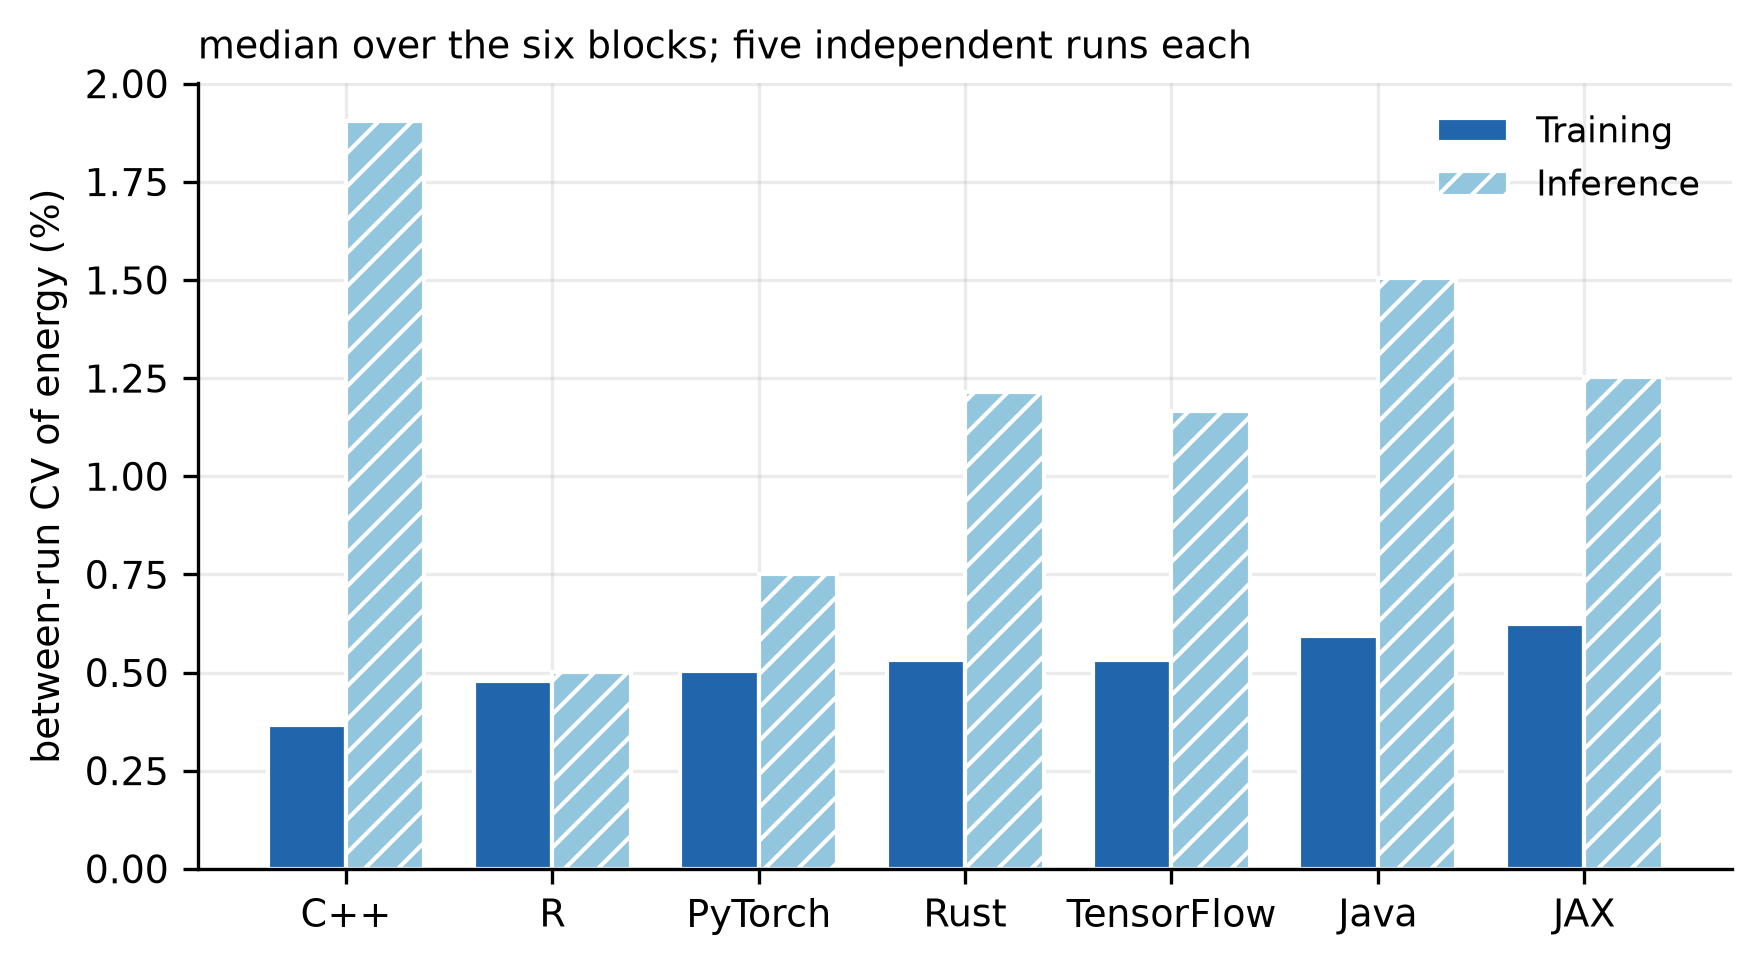
\includegraphics[width=\linewidth]{figures/fig_repeatability.png}
    \caption{Between-run coefficient of variation of energy, median over the six
    (model, dataset) blocks, from \vRepetitions{} independent runs per
    configuration.}
    \label{fig:repeatability}
\end{figure}

Two things follow. First, differences of a few percent between ecosystems are
resolvable, and the differences we report below are far larger than that.
Second, the run-to-run variability is small enough that a single run per
configuration would have produced a plausible-looking number --- which is
precisely why a single run per configuration is not evidence that the number is
right. Low variance is a property of the measurement, not a guarantee about the
thing measured.

\subsection{RQ1: Impact of ecosystems on training energy efficiency}
\label{subsec:rq1}

Figure~\ref{fig:energy_ci} and Table~\ref{tab:train_energy} report training
energy per epoch for every ecosystem and block, at a common chip-level boundary.

\begin{figure*}[t]
    \centering
    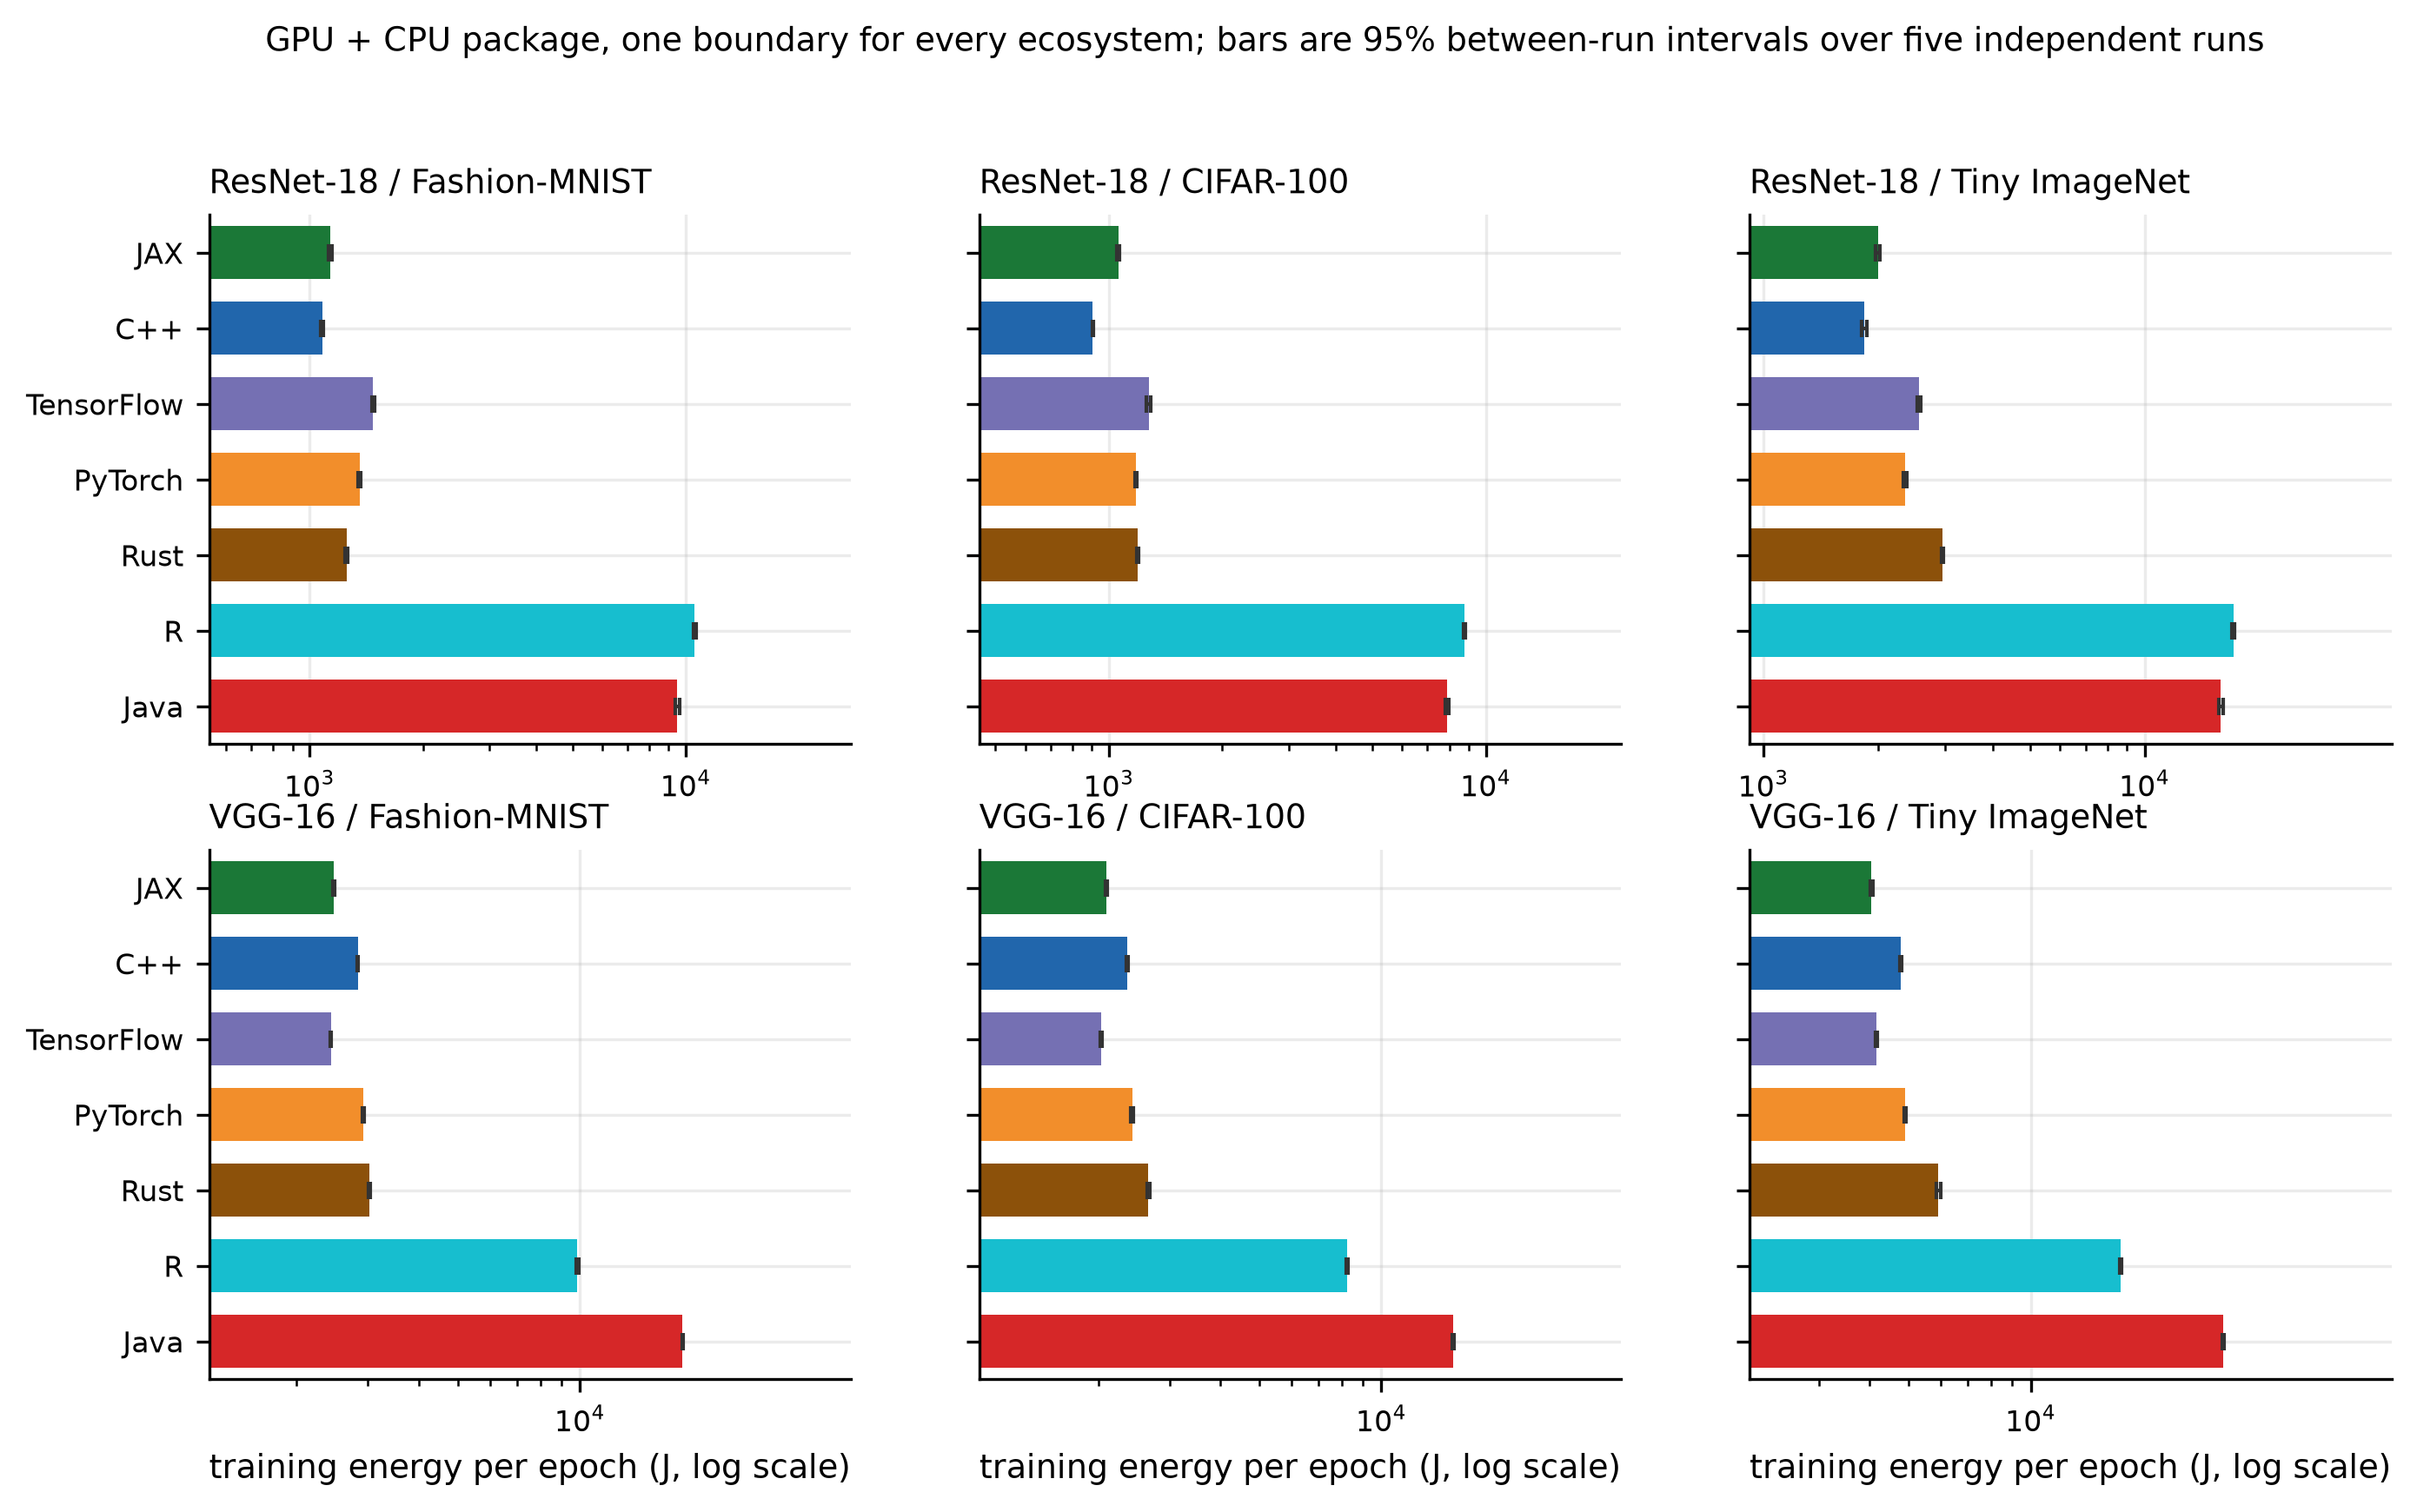
\includegraphics[width=\linewidth]{figures/fig_energy_ci.png}
    \caption{Training energy per epoch, accelerator plus CPU package, with 95\%
    between-run intervals. Note the logarithmic axis: the intervals are narrow
    enough to be hard to see at this scale.}
    \label{fig:energy_ci}
\end{figure*}

\begin{table*}[t]
\centering
\caption{Mean training energy per epoch (J), accelerator plus CPU package.}
\label{tab:train_energy}
% generated by results/analysis/12_paper_numbers.py -- do not edit
\begin{tabular}{lrrrrrr}
\toprule
\textbf{Ecosystem} & \multicolumn{3}{c}{\textbf{ResNet-18}} & \multicolumn{3}{c}{\textbf{VGG-16}} \\
\cmidrule(lr){2-4}\cmidrule(lr){5-7}
 & CIFAR-100 & F-MNIST & Tiny-IN & CIFAR-100 & F-MNIST & Tiny-IN \\
\midrule
C++ & 906 & 1\,080 & 1\,838 & 2\,355 & 2\,833 & 4\,768 \\
JAX & 1\,058 & 1\,132 & 1\,996 & 2\,094 & 2\,471 & 4\,044 \\
PyTorch & 1\,178 & 1\,358 & 2\,359 & 2\,426 & 2\,917 & 4\,898 \\
Rust & 1\,193 & 1\,254 & 2\,948 & 2\,660 & 3\,021 & 5\,918 \\
TensorFlow & 1\,274 & 1\,474 & 2\,559 & 2\,033 & 2\,433 & 4\,164 \\
Java & 7\,904 & 9\,488 & 15\,848 & 15\,029 & 17\,910 & 29\,855 \\
R & 8\,792 & 10\,563 & 17\,087 & 8\,228 & 9\,852 & 16\,646 \\
\bottomrule
\end{tabular}

\end{table*}

The spread between the cheapest and the most expensive ecosystem ranges from
\vSpreadTrainMin$\times$ to \vSpreadTrainMax$\times$ depending on the block
(Table~\ref{tab:spread}), with \vSpreadTrainBest{} cheapest in every one.
This is a substantially larger effect than the 4.6$\times$ an epoch-averaged,
single-run, mixed-boundary analysis of a campaign of this shape would report,
and it is larger for a straightforward reason: once every stack is measured at
the same boundary, the constant host term that used to be added to all of them
--- compressing their ratios toward one --- is gone.

\begin{table}[t]
\centering
\caption{Cheapest and most expensive ecosystem per block, training energy per epoch.}
\label{tab:spread}
\resizebox{\columnwidth}{!}{% generated by results/analysis/12_paper_numbers.py -- do not edit
\begin{tabular}{llrlrr}
\toprule
\textbf{Model} & \textbf{Dataset} & \multicolumn{2}{c}{\textbf{Lowest}} & \multicolumn{2}{c}{\textbf{Highest}} \\
\cmidrule(lr){3-4}\cmidrule(lr){5-6}
 & & {J} & & {J} & {Ratio} \\
\midrule
ResNet-18 & CIFAR-100 & JAX & 617 & R & 9\,619 (15.6$\times$) \\
ResNet-18 & Fashion-MNIST & JAX & 678 & R & 12\,967 (19.1$\times$) \\
ResNet-18 & Tiny ImageNet & JAX & 1\,921 & R & 20\,053 (10.4$\times$) \\
VGG-16 & CIFAR-100 & JAX & 2\,115 & Java & 16\,719 (7.9$\times$) \\
VGG-16 & Fashion-MNIST & JAX & 2\,535 & Java & 20\,094 (7.9$\times$) \\
VGG-16 & Tiny ImageNet & JAX & 4\,287 & Java & 33\,534 (7.8$\times$) \\
\bottomrule
\end{tabular}
}
\end{table}

\textbf{The shared-backend control group.} Four of the \vEcosystems{} ecosystems
run on LibTorch, and three of those four --- Python, C++ and Rust --- train the
byte-identical TorchScript module under specification S1. Whatever separates
them cannot be the kernels, because the kernels are the same code; it is binding
overhead, data movement and host-side dispatch.
Table~\ref{tab:libtorch_control} reports the spread within that group against
the spread across all \vEcosystems{}. A large control-group spread would mean
the effect is host-side rather than intrinsic to the framework; a small one
means the framework choice genuinely dominates.

\begin{table}[t]
\centering
\caption{Spread within the shared-backend control group against the full spread,
per block. The control group holds LibTorch, the model and the data pipeline
fixed.}
\label{tab:libtorch_control}
\resizebox{\columnwidth}{!}{% generated by results/analysis/12_paper_numbers.py -- do not edit
\begin{tabular}{llrrrr}
\toprule
\textbf{Model} & \textbf{Dataset} & \textbf{All 7} & \textbf{Shared module (3)} & \textbf{LibTorch family (4)} & \textbf{Share of log spread} \\
\midrule
ResNet-18 & CIFAR-100 & 14.9$\times$ & 3.8$\times$ & 9.6$\times$ & 49\% \\
ResNet-18 & Fashion-MNIST & 18.2$\times$ & 3.8$\times$ & 10.8$\times$ & 46\% \\
ResNet-18 & Tiny ImageNet & 10.2$\times$ & 3.2$\times$ & 8.5$\times$ & 51\% \\
VGG-16 & CIFAR-100 & 7.9$\times$ & 1.1$\times$ & 1.7$\times$ & 5\% \\
VGG-16 & Fashion-MNIST & 7.9$\times$ & 1.1$\times$ & 1.9$\times$ & 4\% \\
VGG-16 & Tiny ImageNet & 7.8$\times$ & 1.4$\times$ & 1.8$\times$ & 17\% \\
\bottomrule
\end{tabular}
}
\end{table}

\textbf{Energy at equal quality.} A fixed-budget comparison rewards a stack for
learning less. Because every ecosystem now records test accuracy per epoch, we
can check whether it is doing so. Table~\ref{tab:accuracy} reports final test
accuracy by ecosystem and dataset. On Fashion-MNIST all \vEcosystems{} stacks
land within \vAccSpreadFashion{} percentage points of one another
(\vAccMinFashion--\vAccMaxFashion\,\%), which is the strongest available
evidence that they are running the same experiment --- and a check the submitted
design could not perform, because no ecosystem wrote its accuracy to disk. On
the harder datasets the stacks separate more (CIFAR-100:
\vAccMinCifar--\vAccMaxCifar\,\%), and there the energy comparison must be read
alongside the accuracy reached rather than instead of it.

\begin{table}[t]
\centering
\caption{Final test accuracy (\%) after the fixed epoch budget, mean over
\vRepetitions{} runs.}
\label{tab:accuracy}
\resizebox{\columnwidth}{!}{% generated by results/analysis/12_paper_numbers.py -- do not edit
\begin{tabular}{lrrr}
\toprule
\textbf{Ecosystem} & \textbf{Fashion-MNIST} & \textbf{CIFAR-100} & \textbf{Tiny ImageNet} \\
\midrule
C++ & 91.30 & 30.98 & 11.60 (14.37) \\
Java & 91.03 & 20.27 (28.52) & 10.23 (12.66) \\
JAX & 91.36 & 30.56 & 15.19 \\
PyTorch & 91.19 & 31.23 & 12.99 (14.37) \\
TensorFlow & 90.98 & 22.79 (28.24) & 11.31 (14.02) \\
R & 91.64 & 33.34 & 16.57 \\
Rust & 91.12 & 30.81 & 14.74 \\
\bottomrule
\end{tabular}
}
\end{table}

\begin{figure*}[t]
    \centering
    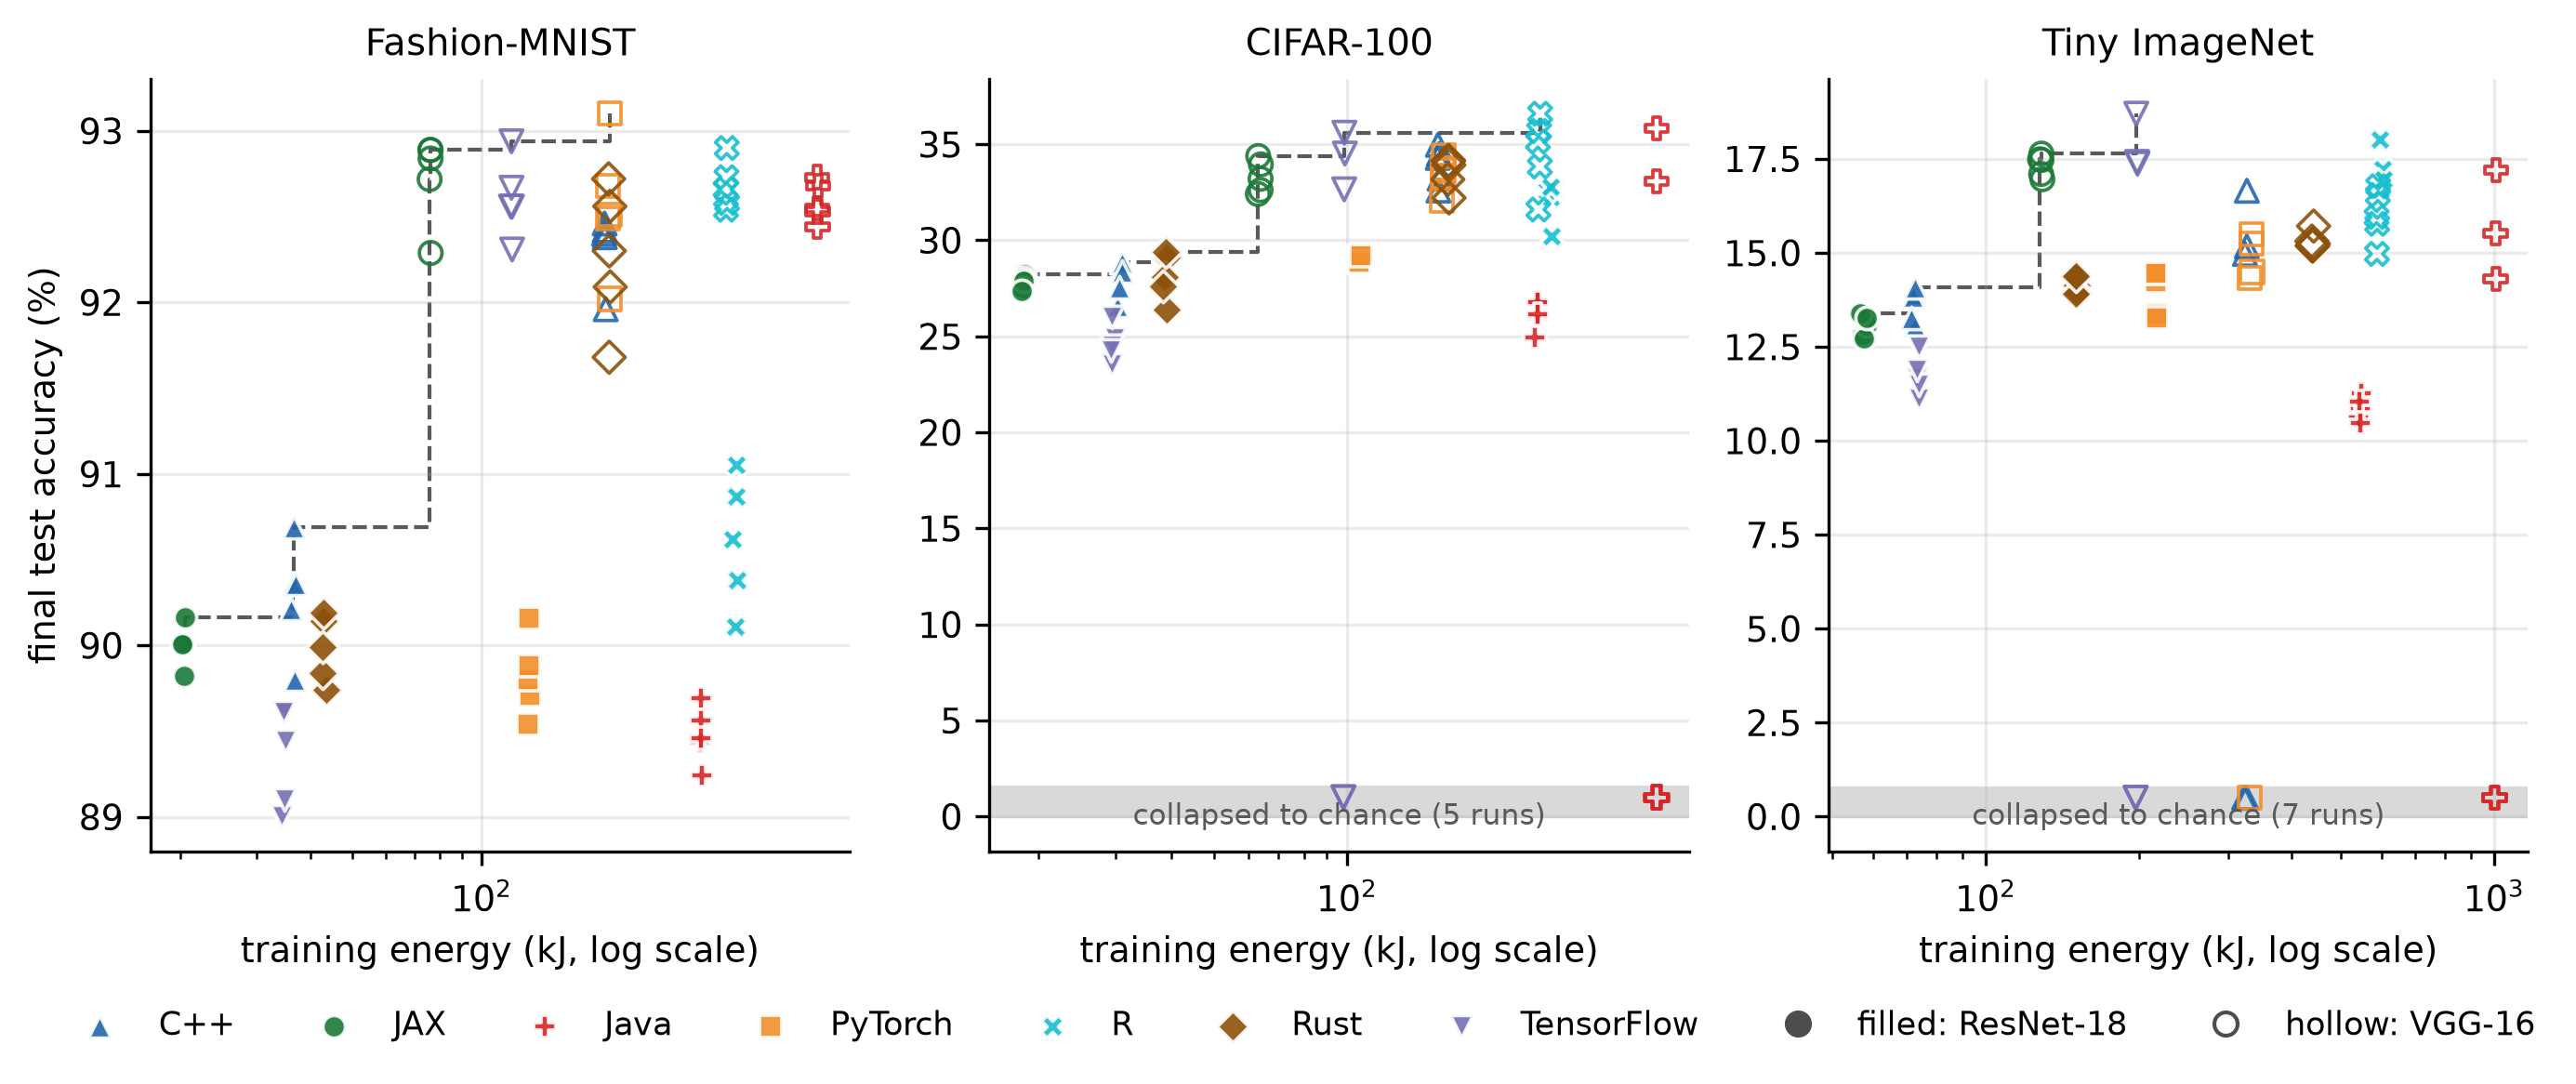
\includegraphics[width=\linewidth]{figures/fig_energy_accuracy.png}
    \caption{Energy spent against accuracy reached, one point per run. The
    dashed line is the empirical frontier: no configuration to its left reaches
    the same accuracy for less energy.}
    \label{fig:energy_accuracy}
\end{figure*}

Figure~\ref{fig:energy_accuracy} plots the two together. Ranking ecosystems by
accuracy per kilojoule rather than by energy alone puts \vEffBest{} ahead of
\vEffWorst{} by \vEffRatio$\times$ --- a different quantity from the energy
ratio, and the one a practitioner choosing a stack actually faces.

\begin{tcolorbox}[colback=gray!5!white, colframe=gray!40!black, title=\textbf{RQ1 Findings: Impact of Ecosystems on Training Energy Efficiency}]
\small
Measured at a common chip-level boundary and replicated \vRepetitions{} times
per configuration, training energy differs across ecosystems by
\vSpreadTrainMin$\times$ to \vSpreadTrainMax$\times$ depending on architecture
and dataset, with \vSpreadTrainBest{} cheapest in every block. Between-run
variability is small (median CV \vCVTrainMedian\,\%), so these differences are
well resolved. Final accuracy converges to within \vAccSpreadFashion{}
percentage points on Fashion-MNIST, so the differences are energetic rather than
qualitative --- the stacks are doing the same work at very different cost.
\end{tcolorbox}

\subsection{RQ2: Impact of ecosystems on inference energy efficiency}
\label{subsec:rq2}

Table~\ref{tab:infer_energy} reports inference energy per epoch over the test
set, at the same boundary.

\begin{table*}[t]
\centering
\caption{Mean inference energy per evaluation pass (J), accelerator plus CPU package.}
\label{tab:infer_energy}
% generated by results/analysis/12_paper_numbers.py -- do not edit
\begin{tabular}{lrrrrrr}
\toprule
\textbf{Ecosystem} & \multicolumn{3}{c}{\textbf{ResNet-18}} & \multicolumn{3}{c}{\textbf{VGG-16}} \\
\cmidrule(lr){2-4}\cmidrule(lr){5-7}
 & CIFAR-100 & F-MNIST & Tiny-IN & CIFAR-100 & F-MNIST & Tiny-IN \\
\midrule
JAX & 68 & 51 & 150 & 121 & 113 & 239 \\
TensorFlow & 73 & 58 & 156 & 136 & 137 & 257 \\
C++ & 81 & 57 & 151 & 193 & 188 & 259 \\
Rust & 113 & 95 & 391 & 313 & 295 & 619 \\
PyTorch & 229 & 252 & 388 & 366 & 363 & 487 \\
Java & 588 & 584 & 616 & 1\,150 & 1\,146 & 1\,155 \\
R & 2\,411 & 2\,676 & 2\,672 & 2\,349 & 2\,629 & 2\,633 \\
\bottomrule
\end{tabular}

\end{table*}

The inference spread is wider than the training spread
(\vSpreadInferMin$\times$ to \vSpreadInferMax$\times$), and this is where the
apparatus matters most. An inference pass at these dataset sizes takes well
under a second in the fastest stacks, which places it below the reported-window
floor characterised in Section~\ref{sec:instrument}. Any inference comparison
drawn from an estimator's own duration field is therefore comparing floors
rather than phases for exactly the stacks that are fastest. Our figures are
counter-bracketed and do not have this problem, but the point generalises: the
inference phase is where a cross-ecosystem energy study is most exposed to its
instrument, and it is also the phase practitioners deploy.

\begin{tcolorbox}[colback=gray!5!white, colframe=gray!40!black, title=\textbf{RQ2 Findings: Impact of Ecosystems on Inference Energy Efficiency}]
\small
Inference energy spreads more widely across ecosystems than training energy
(\vSpreadInferMin$\times$--\vSpreadInferMax$\times$), and does so on blocks short
enough that the measurement instrument, not the ecosystem, becomes the dominant
source of error in a naive design. Reported inference rankings should be treated
as claims about the apparatus until the window over which energy was accumulated
is stated.
\end{tcolorbox}

\subsection{RQ3: Energy--time relationship across ecosystems}
\label{subsec:rq3}

The claim that ``faster is not greener'' is a claim about two measurements, and
it is only as good as the weaker of them. We therefore recompute it on
counter-bracketed durations --- the interval between the two counter reads that
bracket a phase --- rather than on any duration reported by the estimator.

On that basis, energy and time rank the configurations almost identically:
Spearman $\rho = \vRhoTrain$ for training and $\vRhoInfer$ for inference, with
\vDiscordantTrainPct\,\% and \vDiscordantInferPct\,\% of configuration pairs
discordant respectively. Within this workload and platform, execution time is a
good proxy for energy, and the interesting question is why an analysis of the
same experimental shape can conclude otherwise.

The answer is in Figure~\ref{fig:window_floor}. Panel (a) plots the duration
CodeCarbon reports for each block against the counter-bracketed phase. Above
roughly four seconds the two coincide to \vWindowExcessLongMs\,ms. Below it, the
reported duration is a constant: $\max(\text{phase},\ \vWindowFloorS\,\text{s})$
accounts for $R^2 = \vWindowModelRsq$ of its variance. The shortest phase in the
campaign takes \vShortestPhaseS\,s and is filed as \vShortestPhaseReportedS\,s,
a factor of \vShortestPhaseFactor.

\begin{figure*}[t]
    \centering
    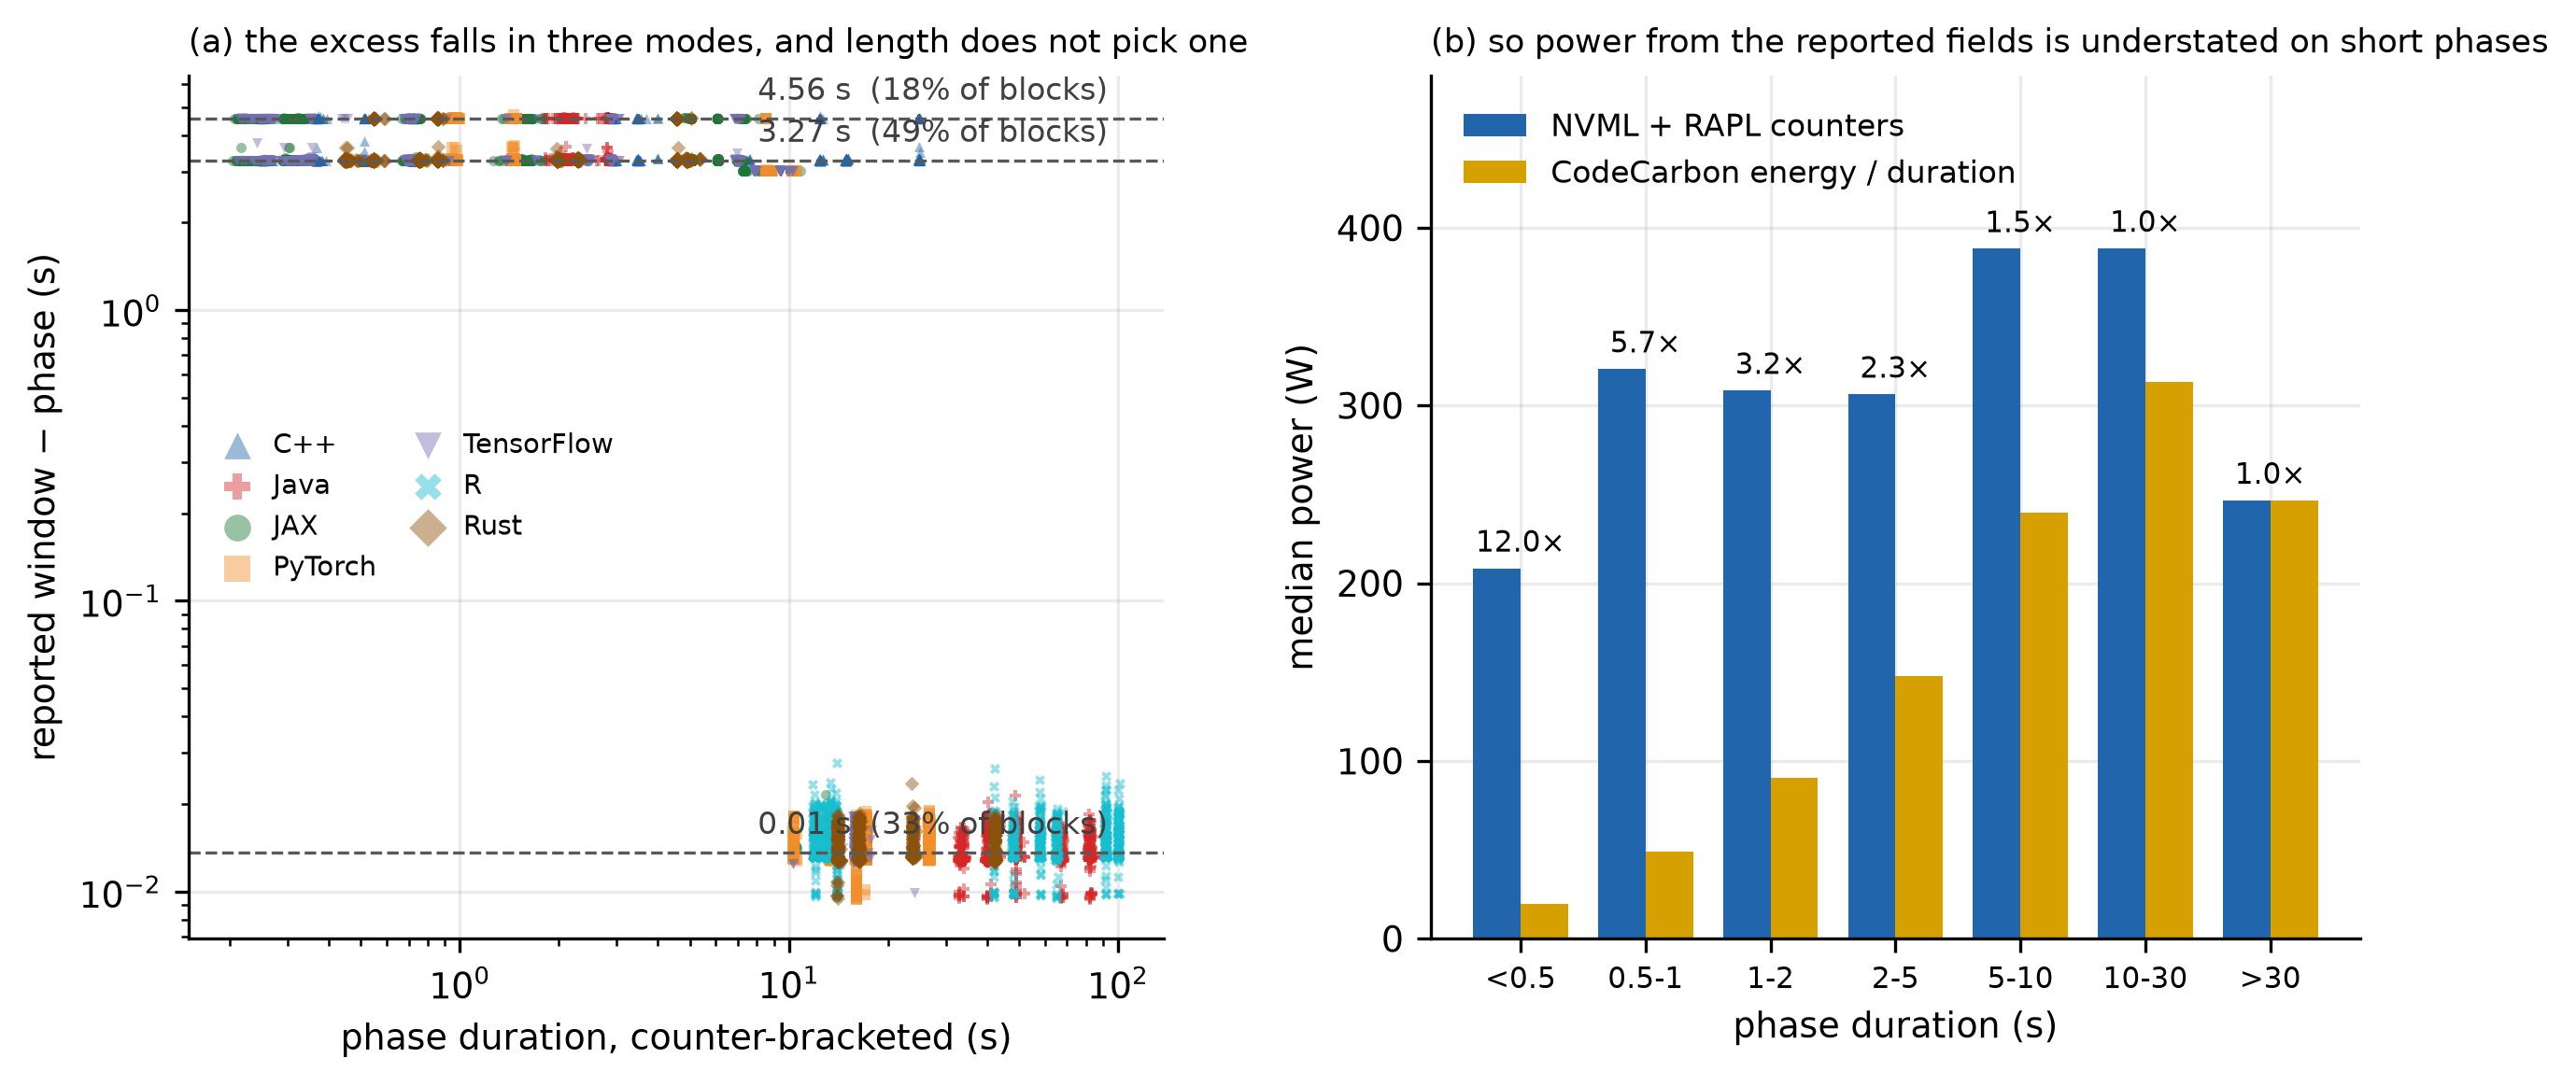
\includegraphics[width=\linewidth]{figures/fig_window_floor.png}
    \caption{(a) The duration reported alongside each energy figure is not the
    interval the energy was accumulated over: it is the phase duration or a
    floor of about four seconds, whichever is larger.
    (b) Power obtained by dividing reported energy by reported duration is
    consequently understated for short phases and exact for long ones.}
    \label{fig:window_floor}
\end{figure*}

Panel (b) shows the consequence. Power computed as reported energy over reported
duration is understated by \vPowerUnderstatedSubSecond$\times$ for sub-second
phases (\vPowerCodeCarbonSubSecond\,W against a measured
\vPowerCountersSubSecond\,W) and is accurate to \vPowerAgreeLongPct\,\% above ten
seconds. The bias is not random and it is not uniform: it is a monotone function
of phase length, so it falls hardest on the fastest ecosystems and on the
inference phase, and it stretches their apparent time axis while leaving their
energy untouched. That is precisely the shape of an artefactual ``fast but
energy-hungry'' finding.

\begin{tcolorbox}[colback=gray!5!white, colframe=gray!40!black, title=\textbf{RQ3 Findings: Energy and Time}]
\small
On counter-bracketed durations, energy and execution time rank ecosystems almost
identically ($\rho = \vRhoTrain$ training, $\vRhoInfer$ inference): within this
workload, faster \emph{is} greener. The contrary finding is reproducible as an
instrument artefact --- the duration field of a widely used software estimator
has a floor of about \vWindowFloorS\,s, which inflates the apparent runtime of
short phases by up to \vShortestPhaseFactor$\times$ while leaving their energy
correct.
\end{tcolorbox}

\subsection{RQ4: How much of this is the apparatus?}
\label{sec:instrument}

Every block in the campaign carries two independent energy readings over the
same window. Figure~\ref{fig:instrument} and Table~\ref{tab:instrument} report
what they say about each other.

\begin{figure*}[t]
    \centering
    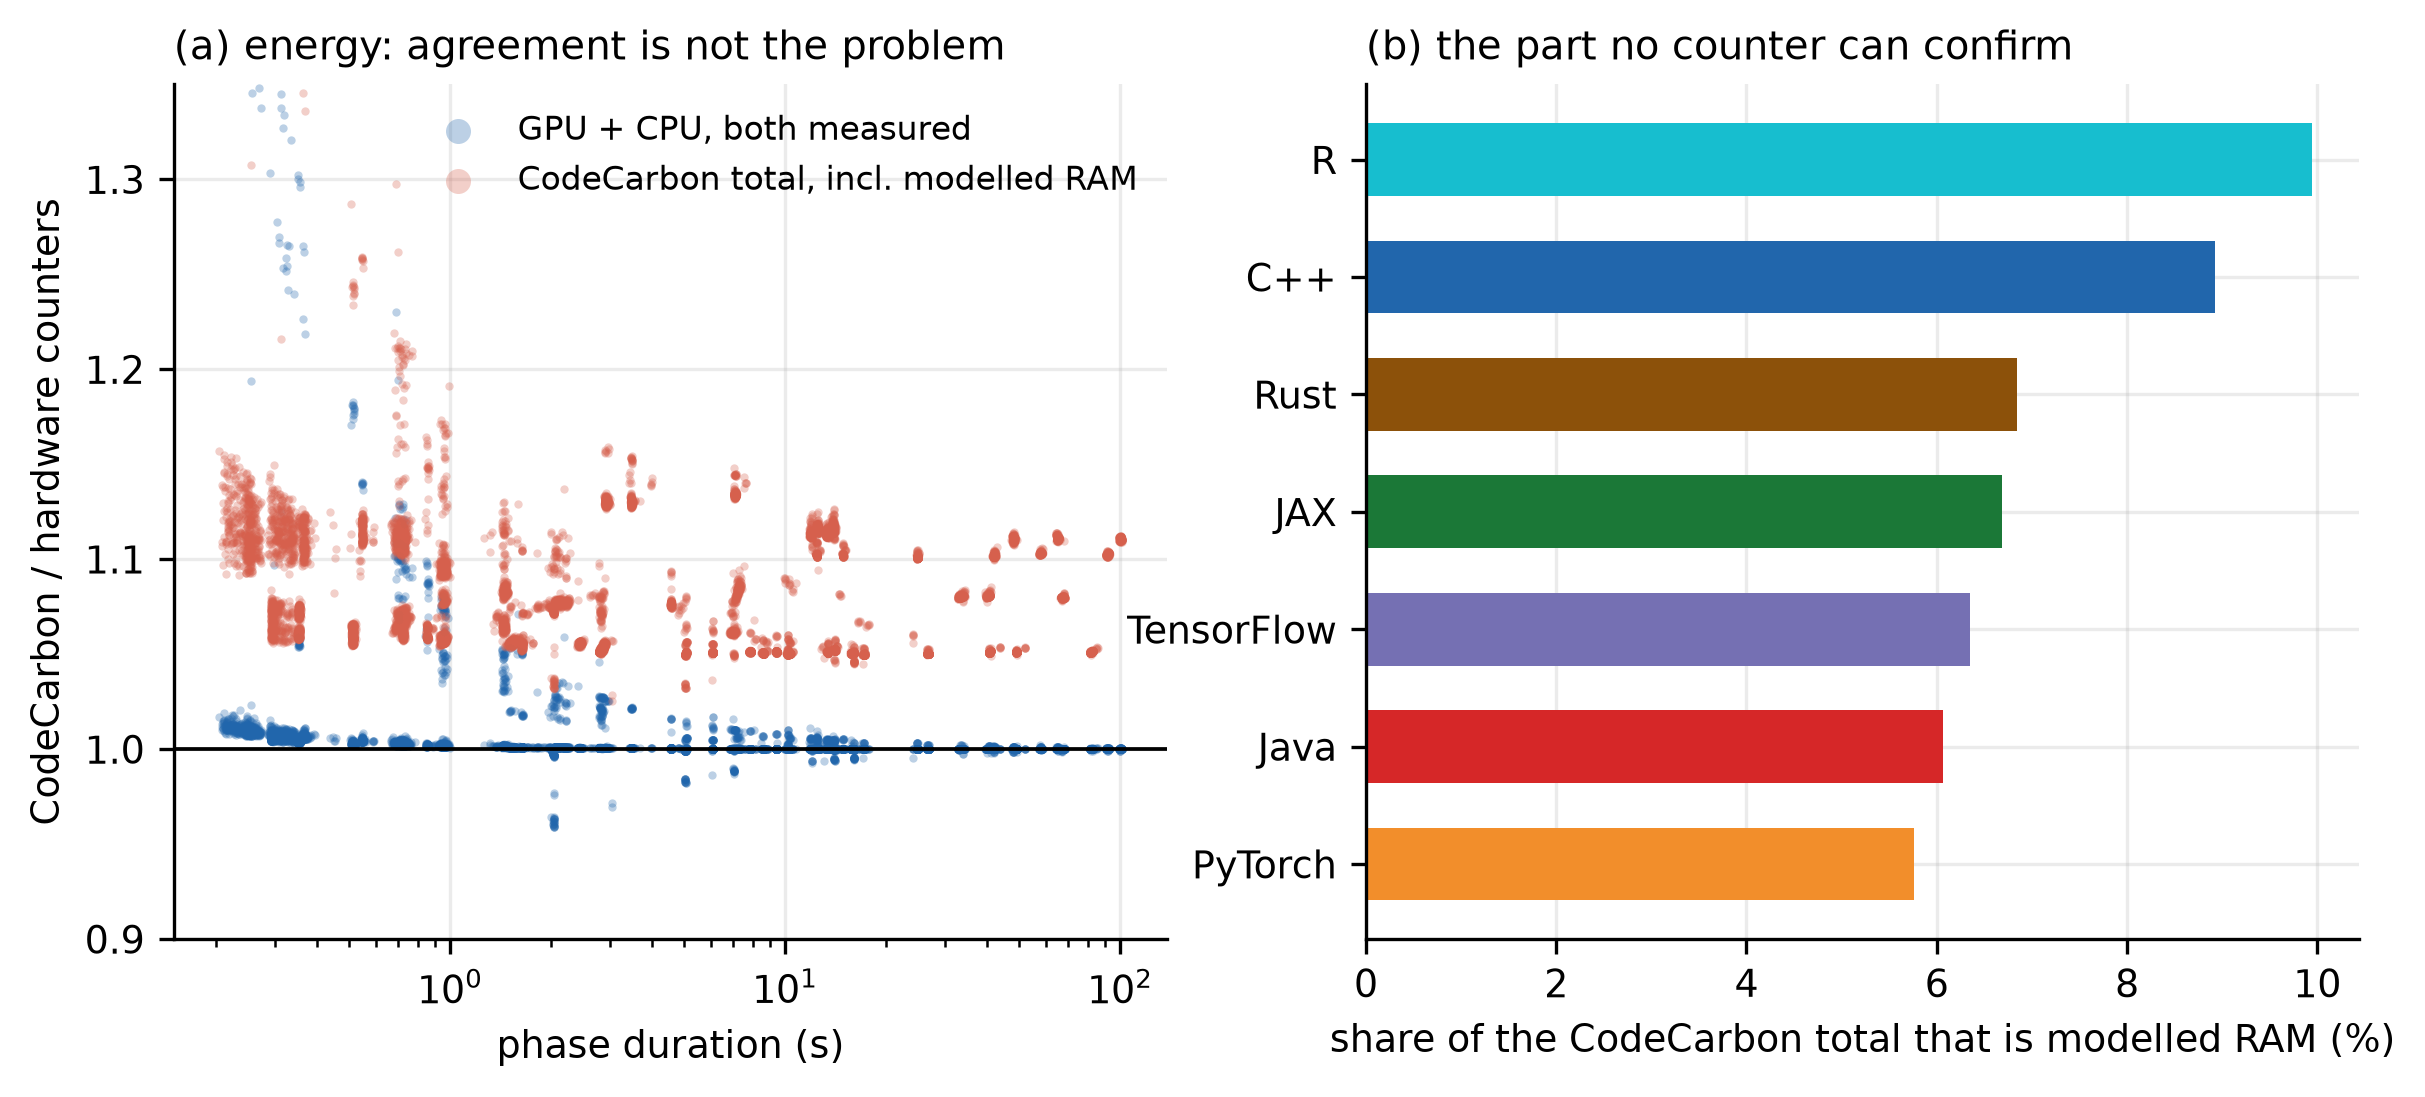
\includegraphics[width=\linewidth]{figures/fig_instrument.png}
    \caption{(a) Ratio of CodeCarbon to hardware counters, per block, against
    phase duration. The measured part agrees; the total does not, by exactly the
    modelled RAM term. (b) The share of each ecosystem's reported total that is
    modelled RAM.}
    \label{fig:instrument}
\end{figure*}

\begin{table}[t]
\centering
\caption{Agreement between the two instruments over \vBlocks{} blocks.}
\label{tab:instrument}
\resizebox{\columnwidth}{!}{% generated by results/analysis/12_paper_numbers.py -- do not edit
\begin{tabular}{lrrr}
\toprule
\textbf{Quantity} & \textbf{Mean} & \textbf{5th pct} & \textbf{95th pct} \\
\midrule
GPU (NVML counter vs CodeCarbon pynvml sampling) & 1.004 & 1.000 & 1.006 \\
CPU package (RAPL counter vs CodeCarbon) & 1.007 & 1.000 & 1.030 \\
GPU + CPU, the measured part & 1.005 & 1.000 & 1.011 \\
CodeCarbon total incl. modelled RAM & 1.084 & 1.050 & 1.131 \\
RAM share of the CodeCarbon total & 7.265 & 4.786 & 10.625 \\
\bottomrule
\end{tabular}
}
\end{table}

\textbf{On energy, the instruments agree.} Over the whole campaign the ratio of
CodeCarbon to counters is \vCCgpuRatio{} for the accelerator and
\vCCcpuRatio{} for the CPU package, or \vCCmeasRatio{} for their sum: a
disagreement of \vCCmeasDisagreementPct\,\%. This is a useful and, we think,
under-reported result. The literature's concern with software estimators is
accuracy, and on this platform, over this workload, with both counters
available, accuracy is not the problem.

\textbf{On what is not measured, they cannot agree.} CodeCarbon's total exceeds
the counters by \vCCtotalRatio$\times$, and the excess is entirely its RAM term
--- \vCCramSharePct\,\% of its reported total on average --- which is derived
from installed memory capacity rather than from memory activity. No counter on
this platform can confirm or refute it. The number is not wrong so much as it is
not a measurement, and it is added silently to a figure otherwise composed of
measurements. On a machine with more installed RAM the same model contributes a
larger share, which means the reported energy of an identical workload depends
on how much memory the host happens to have.

\textbf{Does the instrument change the answer?} We recomputed the ecosystem
ranking of each block under both instruments. They agree in \vRankIdentical{} of
\vRankBlocks{} blocks. The disagreements are confined to adjacent pairs that the
statistical tests do not separate, so the instrument does not reorder the
substantive conclusions of RQ1 --- provided energy, and not power or time
derived from energy, is the quantity being compared.

\begin{tcolorbox}[colback=gray!5!white, colframe=gray!40!black, title=\textbf{RQ4 Findings: The Apparatus}]
\small
Over \vBlocks{} doubly instrumented blocks, a widely used software estimator
agrees with hardware energy counters to \vCCmeasDisagreementPct\,\% on the
quantity both measure, and the ecosystem ranking is unchanged in
\vRankIdentical{} of \vRankBlocks{} blocks. The failure modes lie elsewhere:
a modelled RAM term contributing \vCCramSharePct\,\% of the reported total that
no counter can check and that scales with installed memory rather than with use,
and a reported duration that is a floor rather than a measurement. Both produce
plausible numbers; neither is visible without a second instrument.
\end{tcolorbox}

\section{Discussion}
\label{sec:discussion}

Our study highlights that the energy efficiency of DL workloads is not only a matter of algorithmic or hardware design, but is also materially influenced by the \emph{choice of language--framework ecosystem} (i.e. the adopted stack, including frameworks/libraries, runtimes, and toolchains)~\cite{georgiou2022green,marini2025green,pereira2021ranking,gordillo2024ranking}.
In this section, we interpret the results in light of their broader implications, and discuss lessons learned for different stakeholders.

\subsection{Interpretation of Results}
The experiments reveal three main insights.

\textbf{Phase-dependent rankings.}
First, our results show that efficiency rankings are phase-dependent: ecosystems that are highly efficient during training are not necessarily the most efficient during inference.
In our setting, the Rust ecosystem attains the lowest mean energy consumption during training, whereas during inference the C++ ecosystem dominates, and Rust does not retain its training advantage.
This indicates that optimizations (and overheads) can manifest differently across lifecycle phases, motivating phase-aware decisions rather than a single global ranking.

\textbf{Ecosystem-level overheads amplify with workload scale.}
Second, we observed that higher-consumption ecosystems (e.g. TensorFlow, Java, R in our experiments) exhibit substantially higher energy usage under the same fixed-budget protocol, and that differences tend to become more pronounced as workload complexity increases.
While the exact causes cannot be isolated in a black-box study (they may include runtime layers, input pipelines, execution engines, backend kernel selection, and toolchain differences), the practical implication is clear: ecosystem overheads can become a first-order term at larger scales.
Accordingly, these results should be interpreted as \emph{ecosystem-level} effects rather than attributed to the programming language alone.

\textbf{Energy--time divergence.}
Third, our data reveals a clear \emph{energy--time divergence}: faster execution does not guarantee lower energy consumption.
This reinforces previous warnings against using execution time as a proxy for energy in sustainability evaluations~\cite{weber2023twins,cruz2025greening}.
Taken together, the results suggest that energy usage is shaped not only by runtime, but by how each ecosystem exercises the full stack (framework execution, scheduling/compilation, libraries, and toolchain) under realistic conditions.

\subsection{Implications for Stakeholders}
Our findings carry different implications for different communities:

\begin{itemize}
 \item \textbf{Researchers:} Our results reinforce the need to treat energy as a primary evaluation metric, complementing accuracy and runtime~\cite{schwartz2020green,verdecchia2023systematic,cruz2025greening}.
 Neglecting energy, or using runtime as its proxy, can lead to misleading conclusions about efficiency, especially when comparing heterogeneous ecosystems.

 \item \textbf{Practitioners:} Developers face phase-specific trade-offs.
 In our results, the most energy-efficient ecosystem for training is not the most efficient for inference, implying that "one stack for everything" can be suboptimal when workloads are inference-heavy or training-heavy.
 In practice, ecosystem choice must balance \emph{environmental sustainability} (i.e. energy/time efficiency under the target phase mix) with \emph{organizational sustainability} (i.e. developer skill sets, tooling, long-term maintainability).
 Notably, some widely adopted ecosystems can also be competitive in efficiency in our setting (e.g. PyTorch), but this should not be assumed as a general rule across hardware and toolchains~\cite{georgiou2022green,marini2025green}. 

 \item \textbf{Framework designers:} The results highlight that efficiency stems from the \emph{ecosystem} as a whole (kernels, runtime engines, data pipeline, and toolchain compatibility), not from the surface language alone.
 Therefore, delivering sustainable DL tooling requires attention to end-to-end stack engineering (and reproducible profiling) rather than focusing solely on API design.
 Our pilot attempt to include Julia, which we excluded due to persistent technical issues, illustrates a pragmatic barrier: without sufficient ecosystem stability, potential benefits (including energy efficiency) remain difficult to realize in practice.

 \item \textbf{Policy makers and funding agencies:} AI efficiency is a multifaceted construct involving trade-offs between accuracy, speed, energy, dataset complexity, and lifecycle phase.
 We caution against adopting any single metric (including our Efficiency Index) as a target (Goodhart's Law).
 Instead, policy should promote transparency via multi-dimensional reporting (e.g. separate energy/time for training and inference, accuracy, hardware/software stack details, and toolchain versions) to ensure results are comparable and auditable~\cite{henderson2020systematic,dodge2022efficient,kaack2022aligning}.
\end{itemize}

\subsection{AI Requires Explicit Energy Measurement}
\label{sec:explicit_measurement}

Our results show that ecosystem selection is not a neutral engineering choice, but a factor that can shift deep learning energy consumption by multiple factors in our setting (up to about 4.6$\times$ during training and 7.3$\times$ during inference, depending on the compared ecosystems).
This study provides repeated empirical evidence that \textbf{faster is not always greener}, and that sustainable AI requires explicit measurement of energy, not just accuracy or runtime~\cite{weber2023twins,cruz2025greening,schwartz2020green}.

Furthermore, our findings highlight that efficiency is not only about designing efficient models at a conceptual level, but also about delivering implementations that preserve this efficiency in practice.
Our \emph{black-box evaluation} of off-the-shelf ecosystems is intentional: it reveals differences that would be obscured by hand-tuned or ad-hoc reimplementations, and mirrors how practitioners use frameworks \emph{in vivo}, supporting external validity~\cite{feldt2010validity,ampatzoglou2019identifying,sjoberg2023construct,verdecchia2023threats}.
We also observed that dataset complexity can amplify inefficiencies, meaning sustainability evaluations must consider scaling effects rather than relying on small workloads alone~\cite{tripp2024measuring,banbury2021mlperf}.

Finally, we provide a comprehensive replication package and a fine-grained dataset of our results.
This resource offers concrete evidence and a baseline for framework designers and researchers to diagnose inefficiencies and guide the development of more energy-aware DL ecosystems~\cite{lacoste2019quantifying,verdecchia2023systematic}.


%%%%%%%%%%%%%%%%%%%%%%%%%%%%%%%%%%%%%%%%%%%%%%%%%%%%%%%%%%%%%%%%%%%%%%%%%%%%%%%%%%%%%
%%%%%%%%%%%%%%%%%%%%%%%%%%%%%%%%%%%%%%%%%%%%%%%%%%%%%%%%%%%%%%%%%%%%%%%%%%%%%%%%%%%%%
\subsection{An Industrial Simulation of Deep Green AI Large-Scale Impact}
\label{sec:scenario}

To contextualize our empirical results in a hyperscale setting, we present an illustrative industrial scenario that translates our \emph{relative} ecosystem-level energy differences into approximate energy and cost impacts.
This scenario is not intended as a direct estimate for any specific production system, model family, or hardware stack; rather, it shows how small per-workload gaps can compound at scale.

\textbf{Relative multipliers.}
For a given phase (training or inference) and ecosystem $k$, we define a phase-specific energy multiplier relative to any reference ecosystem $base$ as:
\[
m_k = \frac{\bar{E}_k}{\bar{E}_{\text{base}}},
\]
where $\bar{E}_k$ is the mean energy measured under our experimental protocol for that phase.
Accordingly, $m_k$ should be interpreted as a \emph{relative energy-per-work} factor under our setup, not as a universal constant.

Under the simplifying assumption that the ecosystem-level multiplier transfers to the same workload definition, for any baseline energy budget $\bar{E}_{\text{base}}$, the scaled energy is calculated as $\bar{E}_k = m_k \cdot \bar{E}_{\text{base}}$.

\textbf{Training phase (illustrative scaling).}
From Table~\ref{tab:train_energy}, moving from the most expensive ecosystem in a
block to the cheapest changes training energy by
\vSpreadTrainMin$\times$--\vSpreadTrainMax$\times$. Taking a concrete case: if a
\emph{training} budget is $E=1$~GWh on the most expensive stack of a block, the
same fixed-budget run costs between $1/\vSpreadTrainMax$ and
$1/\vSpreadTrainMin$ of that on the cheapest. At an electricity price of
\SI{100}{\euro\per\mega\watt\hour}~\cite{kaack2022aligning}, the spread between
the two ends of a single block is on the order of hundreds of thousands of euro
per GWh of training. We stress that this is arithmetic on a relative multiplier,
not a forecast: it assumes the multiplier transfers to a workload of a different
size on different hardware, which is exactly the assumption our own measurements
give us the least confidence in.

\textbf{Inference phase (hyperscale workload, fixed work).}
Inference energy scales approximately linearly with served volume when stacks
are compared at a fixed service target. Let $E_{\text{PyTorch}}$ be the daily
energy attributable to \emph{inference} with PyTorch as the baseline. Assuming
$N=100{,}000$ accelerators running continuously for 24 hours at an average
inference-attributable draw of $P=0.4$~kW each gives
$E_{\text{PyTorch}} = \vScenarioBaselineMWh$~MWh/day, or
\vScenarioBaselineCost~\euro\ per day at
\SI{100}{\euro\per\mega\watt\hour}. Applying the measured inference multipliers
yields Table~\ref{tab:industrial_inference}: \vScenarioBest{} at
\vScenarioBestMult$\times$ the baseline and \vScenarioWorst{} at
\vScenarioWorstMult$\times$.

\begin{table*}[t]
\centering
\caption{Projected daily energy and cost for large-scale inference
($10^5$ accelerators, 24\,h, electricity at
\SI{100}{\euro\per\mega\watt\hour}), scaling the \emph{relative} inference
energy measured in this campaign with Python/PyTorch as the baseline. These are
scenario arithmetic on measured multipliers, not forecasts.}
\label{tab:industrial_inference}
\resizebox{0.8\textwidth}{!}{% generated by results/analysis/12_paper_numbers.py -- do not edit
\begin{tabular}{lrrrrr}
\toprule
\textbf{Ecosystem} & \textbf{Accelerator-hours} & \textbf{Fleet} & \textbf{Measured draw} & \textbf{Energy (MWh/day)} & \textbf{Cost (\euro/day)} \\
\midrule
C++ & 0.37$\times$ & 36\,796 & 197\,W & 174 & 17\,365 \\
Rust & 0.68$\times$ & 68\,031 & 190\,W & 311 & 31\,060 \\
TensorFlow & 0.81$\times$ & 81\,069 & 173\,W & 336 & 33\,644 \\
JAX & 0.94$\times$ & 94\,170 & 166\,W & 376 & 37\,560 \\
PyTorch (baseline) & 1.00$\times$ & 100\,000 & 167\,W & 401 & 40\,088 \\
R & 13.22$\times$ & 1\,321\,558 & 121\,W & 3\,850 & 384\,977 \\
Java & 6.06$\times$ & 606\,078 & 265\,W & 3\,859 & 385\,886 \\
\bottomrule
\end{tabular}
}
\end{table*}

\textbf{Takeaway.}
Ecosystem-level energy differences, treated purely as relative multipliers under
a uniform protocol, translate into large operational deltas at hyperscale. Two
caveats bound that statement, and both come from this study rather than from
convention. The multipliers were measured on a single-accelerator desktop at
$32\times32$ input resolution, a regime in which data movement and dispatch
weigh more heavily than they would at production scale, so they are more likely
to overstate binding overhead than to understate it. And the whole calculation
is a scaling of \emph{relative} differences: had we reported the modelled
component of a software estimator's output as if it were measured, the same
arithmetic would have produced a confident number from a quantity that depends
on how much memory the host happens to have.

\section{Threats to Validity}
\label{sec:threats}

As with any empirical study, our work is subject to several threats to validity. In this section we outline the main risks and the measures we adopted to mitigate them, following the classification into internal, construct, external, and conclusion validity~\cite{feldt2010validity,ampatzoglou2019identifying,wyrich2024evidence}. Threats are reported by considering those that might have most deeply \emph{affected} our results, and by acknowledging common pitfalls that may arise while discussing them~\cite{verdecchia2023threats}.

\textbf{Internal Validity.}
A primary threat concerns the execution environment.
Experiments were run on a dedicated high-performance server (cf. Section~\ref{sec:execution}); despite efforts to minimize background processes, residual system activity (e.g. operating system daemons) may still have influenced energy measurements~\cite{verdecchia2023threats}.
We mitigated this risk by isolating workloads and monitoring runs under comparable conditions.

Another internal threat stems from the use of multiple frameworks and toolchains, each relying on different CUDA and cuDNN versions due to compatibility constraints.
For instance, the required CUDA versions in our study ranged from 11.6 (for Java's Deeplearning4j) to 12.8 (for C++'s LibTorch), with corresponding variations in cuDNN libraries (see our replication package for a complete dependency list).
Such heterogeneity can affect both runtime efficiency and energy usage~\cite{patterson2021carbon,marini2025green}, potentially favoring ecosystems with more up-to-date backends.
Although not controlled, this variability reflects the reality practitioners encounter ``in the wild''~\cite{sjoberg2023construct}.
Accordingly, we interpret our results as differences between language--framework ecosystems (including their officially supported runtimes and toolchains), and we avoid attributing the observed effects to the programming language alone.

Implementation choices represent another source of internal threats.
We deliberately avoided ad-hoc optimizations and advanced engineering techniques, preferring instead to configure models and frameworks in ways that closely resemble how a practitioner or applied researcher would use them~\cite{verdecchia2023systematic}.
Specifically, we maintained uniform hyperparameters across all ecosystems.
While we acknowledge that certain ecosystems might benefit from different configurations, we adopt uniform hyperparameters as a controlled fixed-budget comparison across ecosystems (same recipe and number of epochs), which does not guarantee convergence equivalence across frameworks.
Moreover, introducing hyperparameter tuning would introduce a significant \emph{confounding variable}, making it difficult to discern whether differences stem from the ecosystem itself or from the tuning process.

Another example is data loading and preprocessing.
In some community repositories for C++ and Rust we observed unconventional strategies, such as pre-loading the entire dataset into memory to accelerate training.
While effective in reducing runtime, this approach diverges from standard practice and introduces bias.
To preserve comparability, we enforced consistent high-level data loading constraints and standardized final layers to match dataset classes.
Nevertheless, data-loading and preprocessing are not identical across ecosystems (e.g. thread scheduling, host-to-device transfer patterns, and memory allocation strategies), and such differences may contribute to the measured energy and time.
In all cases, we relied on official library implementations or community-accepted baselines~\cite{banbury2021mlperf,tripp2024measuring}.
Some outliers may remain (e.g. MATLAB occasionally exhibited anomalous behavior), and we acknowledge that implementation-level variability may have influenced results.
Finally, all datasets were downloaded and stored locally, avoiding network access or web-based loaders that could introduce additional overhead.

GPU-side runtime effects can also introduce additional uncontrolled variability, such as thermal throttling, framework-specific JIT compilation or graph compilation effects.
We partially mitigated this by running on dedicated hardware and averaging measurements over multiple epochs; however, we cannot fully exclude that early-epoch warm-up effects (e.g. memory allocator initialization, autotuning) affect phase-specific measurements.

\textbf{Construct Validity.}
A primary threat to construct validity concerns the operationalization of our target construct, ``sustainability''.
In this work, we used \textbf{energy consumption} (measured in Joules) as its primary proxy.
As argued in Section~\ref{sec:background}, we selected this metric over derived alternatives (e.g. carbon footprint) because it is a direct and reproducible measure of computational effort, less affected by confounding variables such as the grid's energy mix or the geographic location of the server.

A secondary threat concerns the accuracy of measuring this proxy.
Energy consumption was operationalized using the \texttt{CodeCarbon} toolkit~\cite{lacoste2019quantifying}.
While \texttt{CodeCarbon} leverages NVIDIA’s NVML and system profilers, a potential threat is the reliance on software-level sampling rather than external hardware power meters~\cite{patterson2022plateau,cruz2025greening}.
We extended \texttt{CodeCarbon} with a custom daemon to obtain fine-grained, phase-specific measurements (training and inference); nevertheless, absolute values may not perfectly reflect actual power draw.
Although the tracker runs out-of-process and the server was dedicated, we cannot fully exclude minor interference effects (e.g. sampling overhead or scheduling interactions), which we treat as a limitation common to software-based profiling.
Therefore, we primarily interpret measurements as supporting \emph{relative comparisons} under an identical measurement protocol, rather than as precise absolute ground-truth energy values.
Recent validation work comparing estimator-based measurements against external ground-truth reports that established estimation approaches can exhibit errors up to 40\%, and that dynamic estimation can systematically underestimate consumption by about 20--30\% in some settings~\cite{fischer2025groundtruthing}.

Finally, minor adaptations to model implementations (e.g. modifying final classification layers or adopting community loaders) could have introduced variability, potentially confounding the construct.
We mitigated this risk by documenting all changes and ensuring they were minimal and aligned with community practice~\cite{mehlin2023towards,verdecchia2023systematic}.

\textbf{External Validity.}
Our study focused on two convolutional architectures (ResNet-18 and VGG-16) and three image classification datasets (Fashion-MNIST, CIFAR-100, Tiny ImageNet).
While these choices are representative of standard computer vision tasks, results may not generalize to other model families (e.g. transformers, large language models) or other domains (e.g. speech recognition, tabular learning)~\cite{strubell2019energy,patterson2021carbon}.
Similarly, although the chosen languages cover prominent DL ecosystems in current practice, they do not encompass all possible programming environments.
Our selection focuses on mature, GPU-compatible DL ecosystems with stable support from the community or vendor support; conclusions should not be extrapolated to ecosystems not covered by this criterion.

Moreover, we evaluated a specific hardware platform (a single NVIDIA RTX 3090 with an AMD Ryzen 9 5900X); results may vary with different GPUs, CPUs, drivers, or heterogeneous accelerators (e.g. TPUs, embedded devices)~\cite{patterson2022plateau,kaack2022aligning}. A single-accelerator desktop also makes the host share of total energy smaller than it would be on a multi-socket server, which flatters no ecosystem in particular but does bound the generality of the absolute figures.
Nonetheless, our design balances realism and breadth with tractability, and provides a meaningful baseline within the stated ecosystem-level scope~\cite{verdecchia2023systematic}.

\textbf{Conclusion Validity.}
Variability in results could arise from stochastic effects of DL training (e.g. random initialization, non-deterministic GPU operations)~\cite{weber2023twins}.
We mitigated this by standardizing hyperparameters and using fixed seeds where supported, though some frameworks may not guarantee full determinism.

A specific threat to statistical fairness concerns the presence of outliers or abnormal execution cycles in certain ecosystems.
We report arithmetic means over the collected measurements to summarize average behavior under our protocol; however, averages can be sensitive to anomalous execution cycles, and robust estimators (e.g. medians/trimmed means) are left for future work.
Since runtime anomalies (e.g. memory management spikes or non-optimal garbage collection) correspond to real energy consumption that users would incur, their inclusion provides a more faithful and transparent estimation of the total impact.

Moreover, while differences in mean energy consumption are substantial in our setting (e.g. up to about 4.6$\times$ in training and 7.3$\times$ in inference between best and worst ecosystems), smaller differences should be interpreted with caution.
In addition, while we average measurements over epochs, epochs within the same run are not statistically independent; therefore, treating epoch-level measurements as independent samples would inflate statistical confidence.
Additional independent run-level repetitions per configuration would strengthen statistical inference and are left for future work.

In summary, while several threats to validity remain, we believe the precautions adopted---dedicated hardware, consistent hyperparameters (as a fixed-budget recipe), standardized data handling where feasible, phase-specific tracking, and reliance on official or community-accepted implementations---support the robustness and practical relevance of our findings, within the stated ecosystem-level scope~\cite{verdecchia2023threats}.


%%%%%%%%%%%%%%%%%%%%%%%%%%%%%%%%%%%%%%%%%%%%%%%%%%%%%%%%%%%%%%%%%%%%%%%%%%%%%%%
\section{Conclusion}
\label{sec:conclusion}

This paper presented a case study on the impact of \emph{language--framework ecosystems} on the energy efficiency of \emph{Deep Learning (DL) workloads}, focusing on \emph{computer vision} image classification.
We conducted a systematic experimental campaign across six language-based ecosystems (Python, C++, Java, R, MATLAB, and Rust), eight frameworks/libraries, and three datasets of increasing complexity~\cite{banbury2021mlperf}.
Energy consumption was monitored at fine granularity, enabling separate analyses of training and inference phases~\cite{lacoste2019quantifying,patterson2021carbon}.

Our results highlight three key findings.
First, ecosystem selection can substantially shift operational efficiency in our setting, with gaps reaching about \textbf{11$\times$} in execution time during training and about \textbf{7.3$\times$} in energy consumption during inference (and about \textbf{4.6$\times$} in energy during training).
Importantly, these differences should be interpreted at the ecosystem level (framework execution engines, runtimes, and toolchains), rather than attributed to the programming language alone.

Second, training and inference phases exhibit markedly different efficiency rankings across ecosystems.
This underscores the need to evaluate both lifecycle stages separately---a critical consideration for industrial scenarios and a recurring theme in Green AI research~\cite{cruz2025greening,mehlin2023towards}.

Third, our results repeatedly demonstrate that execution time and energy usage do not always correlate.
This reveals a non-trivial energy--time trade-off and supports our central finding that \textit{faster does not imply greener}, confirming similar warnings from related software engineering domains~\cite{weber2023twins,verdecchia2023systematic}.

Overall, these findings stress that ecosystem selection---often treated as a secondary engineering decision---can have significant sustainability implications~\cite{schwartz2020green,verdecchia2023systematic,kaack2022aligning}.
For practitioners, this suggests that energy-aware ecosystem choices can yield substantial savings at scale, especially when the expected phase mix (training- and inference-heavy) is made explicit~\cite{patterson2022plateau,cruz2025greening}.
For researchers, our study motivates further investigation of the intersection between Green AI and software engineering practices, with an emphasis on reproducible ecosystem-level benchmarking and phase-aware evaluation~\cite{schwartz2020green,verdecchia2023systematic,cruz2025greening}.


%%%%%%%%%%%%%%%%%%%%%%%%%%%%%%%%%%%%%%%%%%%%%%%%%%%%%%%%%%%%%%%%%%%%%%%%%%%%%%%
\section{Future Work}
\label{sec:future}

Building on this study, several promising directions remain open.

First, our analysis can be extended to more diverse model families beyond CNNs, such as transformers and multimodal architectures, to assess whether the observed ecosystem-level patterns hold under different operator mixes, memory footprints, and compilation strategies~\cite{patterson2021carbon}.

Second, testing on heterogeneous hardware platforms (e.g. TPUs, embedded and edge devices) would clarify how robust the observed rankings are under different accelerator toolchains and runtime stacks~\cite{patterson2022plateau,kaack2022aligning}.
In particular, future work should explicitly treat the \emph{hardware--software stack} as part of the ecosystem definition (driver versions, compiler toolchains, and vendor runtimes), rather than assuming portability of efficiency rankings.

Third, a deeper exploration of the \emph{energy--time trade-off} is needed to identify regimes where faster execution is beneficial or detrimental from a sustainability perspective, including phase-aware serving constraints~\cite{weber2023twins,cruz2025greening}.

Fourth, complementing our black-box, off-the-shelf evaluation, future work could introduce a controlled \emph{white-box} layer-level analysis (e.g. per-layer profiling) implemented with each ecosystem's native primitives.
This would help localize where inefficiencies originate (e.g. convolution/attention kernels, activation and normalization layers, data pipelines, host-to-device transfers, memory allocation and caching), and clarify which components are ecosystem-driven versus model-driven~\cite{georgiou2022green,marini2025green,pereira2021ranking,gordillo2024ranking}.
Crucially, such analysis should be designed as \emph{complementary} evidence, since fine-grained attribution can reduce realism while increasing internal control.

Finally, expanding the scope of reproducibility by incorporating real-world workloads, distributed training and inference (multi-GPU, multi-node), and standardized energy-aware benchmarks would enable evaluation in contexts closer to production environments~\cite{lacoste2019quantifying,verdecchia2023systematic,banbury2021mlperf}.
A particularly valuable extension would be to include independent run-level repetitions (not only epoch-level repeated measurements) and to cross-validate software-based energy estimates with external power sensors in a subset of configurations, to strengthen both statistical inference and measurement validity~\cite{verdecchia2023systematic}.


%%%%%%%%%%%%%%%%%%%%%%%%%%%%%%%%%%%%%%%%%%%%%%%%%%%%%%%%%%%%%%%%%%%%%%%%%%%%%%%

\section{Carbon Footprint of This Study}

The total carbon footprint of our experiments is estimated at approximately 3.3~kg of CO$_2$e, based on  \texttt{CodeCarbon} measurements across 7,200 training and inference epochs. This corresponds to the emissions of driving an average passenger car for about 27~km (17~miles), an equivalency derived from average new car emissions data reported by the European Environment Agency (EEA)~\cite{EEA-cars-monitoring}, or the electricity required to power a typical European household for one day, based on residential energy consumption data from Eurostat~\cite{Eurostat-energy-data}. 
While modest compared to large-scale industrial training, this evaluation underscores the importance of quantifying and reporting the environmental impact of research experiments.


%%%%%%%%%%%%%%%%%%%%%%%%%%%%%%%%%%%%%%%%%%%%%%%%%%%%%%%%%%%%%%%%%%%%%%%%%%%%%%%
\section{Declaration of Generative AI and AI-assisted Technologies in the Writing Process}
During the preparation of this work the authors used ChatGPT-5 in order to improve the readability of the manuscript text. After using this tool, the authors reviewed and edited the content as needed and take full responsibility for the content of the article.

\balance
\bibliographystyle{IEEEtran}
\bibliography{bibliography}


\newpage
%%%%%%%%%%%%%%%%%%%%%%%%%%%%%%%%%%%%%%%%%%%%%%%%%%%%%%%%%%%%%%%%%%%%%%%%%%%%%%%
\bio{bio/leo.jpg}
\textbf{Leonardo Pampaloni} graduated with a Master’s degree in Software Engineering from the University of Florence, Italy, achieving top marks. His research interests lie in software sustainability and energy efficiency in Artificial Intelligence, with particular emphasis on Green AI and computer vision. He has contributed to empirical studies on cross-language benchmarking of AI frameworks and optimization of DL workloads. More information is available at \url{https://github.com/Pampaj7}.
\endbio

\bio{bio/marco.jpg}
\textbf{Marco Pagliocca} received a Bachelor’s degree in Computer Engineering with highest honors from the University of Florence, Italy, where he is currently pursuing a Master’s degree in the same field. His research interests focus on environmental sustainability, human-centered engineering, and the use of technology as a means to improve everyday life. He believes that Artificial Intelligence can simplify mechanical tasks and encourage greater attention to meaningful aspects of human activity.
\endbio

\bio{bio/enrico.jpg}
\textbf{Enrico Vicario} is a Professor of Computer
Science and Engineering and the Head of the Software Technologies Laboratory of the University of Florence, Italy. His research interests include the area of software engineering, with a focus on quantitative evaluation of stochastic models, software architectures and methodologies, and on their connection through model-driven engineering practices.
\endbio

\bio{bio/roberto.jpg}
\textbf{Roberto Verdecchia} is an Assistant Professor at the Software Technologies Laboratory (STLab) of the University of Florence, Italy. He holds a double Ph.D.\ in Computer Science, appointed by the Gran Sasso Science Institute, L'Aquila, Italy, and the Vrije Universiteit Amsterdam, the Netherlands. His research interests focus on the adoption of empirical methods to improve software development and system evolution, with particular interest in the fields of  technical debt, software architecture, software sustainability, and software testing. More information is available at \href{https://robertoverdecchia.github.io/}{robertoverdecchia.github.io}. %He was the recipient of a ACM/SIGSOFT Distinguished Paper Award (ICSE'19)...andt others?.
\endbio

\end{document}